%###############################################################################
%
%
\part{Particle description}
%
%
%###############################################################################

%--------------------------------------------------------------------------------------------------------------------------------------------
\chapter{Classical Mechanics}
%--------------------------------------------------------------------------------------------------------------------------------------------
\begin{table}[H]
\renewcommand{\arraystretch}{1.5}
\centering
\caption{Various coordinates of classical mechanics. }
\label{tb:classical_mechanics_coordinates}
 \begin{tabular}{l|l|l}
    Classical coordinates & $\xvec(t)$ & $\vvec(t)$ \\
    \hline
    Generalized coordinates  & $\qvec$ & $\qvecdot$ \\
    \hline
    Canonical coordinates & $\qvec$ & $\pvec$ \\
    \hline
    Time-dependent canonical coordinates & $\tilde{\qvec}(t)$ & $ \tilde{\pvec}(t)$ \\
 \end{tabular}
\end{table}

\section{Lagrangian mechanics}

\begin{itemize}
\item Define the position $\xvec = \xvec(t)$ and velocity $\vvec = \vvec(t)$ of a particle. 

\item Define the Lagrangian as $L = L(\qvec, \qvecdot,t)$, where $\qvec$ and $\qvecdot$ are the generalized position and generalized velocity, respectively. 

\item The equations of motion are obtained from the Euler-Lagrange equation, which is 
\begin{equation}
\frac{d}{dt} \left [ \left ( \frac{\partial L}{\partial \qdot_i } \right )_{\qvec =  \xvec, \qvecdot = \vvec }  \right] = \left ( \frac{\partial L}{\partial q_i} \right )_{ \qvec =  \xvec, \qvecdot = \vvec} .
\end{equation}

\item For example, the Lagrangian of a particle in an electromagnetic field where $\phi = \phi(\qvec,t)$ is the electric potential and $\Avec = \Avec(\qvec,t)$ is the magnetic potential, is
\begin{equation}
L = \frac{1}{2} m \qdot_i \qdot_i + e \qdot_i A_i - e\phi.
\end{equation}
The derivatives in the Euler-Lagrange equation are
\begin{equation}
\frac{\partial L}{\partial q_i} = e \qdot_j \frac{\partial A_j }{\partial q_i} - e \frac{\partial \phi}{ \partial q_i}
\end{equation}
\begin{equation}
\frac{\partial L}{\partial \qdot_i} = m \qdot_i + e A_i 
\end{equation}
\begin{align}
\frac{d}{dt}\left [ \left ( \frac{\partial L}{\partial \qdot_i } \right )_{\qvec =  \xvec, \qvecdot= \vvec }  \right] &= \frac{d}{dt} \left [ m v_i + e A_i(\xvec,t) \right ] \nonumber \\
&= m \frac{ d v_i}{dt} + e v_j \left (\frac{\partial A_i}{\partial q_j} \right )_{\qvec = \xvec} +  e \left (\frac{\partial A_i}{\partial t} \right )_{\qvec = \xvec} .
\end{align}
Thus, the Euler-Lagrange equation becomes
\begin{equation}
\label{eq:lag_mech_tensor_lorentz}
m \frac{ d v_i}{dt} = \left ( - e v_j \frac{\partial A_i}{\partial q_j} - e\frac{\partial A_i}{\partial t} + e v_j \frac{\partial A_j }{\partial q_i} - e \frac{\partial \phi}{ \partial q_i}\right )_{\qvec = \xvec}.
\end{equation}
In vector notation, this is written as
\begin{equation}
    m \frac{d \vvec}{dt} = \left(-e\vvec \cdot \nabla_q \Avec - e \frac{\partial \Avec}{\partial t} + e \nabla_q (\vvec \cdot \Avec) - e \nabla_q \phi \right)_{\qvec = \xvec}.
\end{equation}
Using the vector identity (4) from Griffiths book, the above can be expressed as
\begin{equation}
m \frac{d\vvec}{dt} = e \left ( \Evec + \vvec \times \Bvec \right)_{\qvec = \xvec},
\end{equation}
where $\Evec = \Evec(\qvec,t)$ and $\Bvec = \Bvec(\qvec,t)$.
\end{itemize}

\section{Hamiltonian mechanics}
\begin{itemize}
\item Define the Hamiltonian as $H = H(\qvec, \pvec, t)$, where $\qvec$ and $\pvec$ are the canonical position and momentum. For all purposes here, the canonical position is the same as the generalized position.

\item The Hamiltonian is obtained from the Lagrangian using
\begin{equation}
H = \left ( \qvecdot \cdot \pvec - L \right)_{\qvecdot = \fvec(\qvec, \pvec)},
\end{equation} 
where the dependency of $\qvecdot$ on $\qvec$ and $\pvec$ is obtained from evaluating
\begin{equation}
\label{eq:v_from_qp}
\pvec = \frac{ \partial L}{\partial \qvecdot}.
\end{equation}

\item For example, for a particle in an electromagnetic field we have
\begin{equation}
H = \left [ \qdot_i p_i - \left ( \frac{1}{2} m \qdot_i \qdot_i + e \qdot_i A_i - e\phi \right ) \right]_{\qvecdot = f(\qvec, \pvec)}. 
\end{equation}
Evaluating \cref{eq:v_from_qp} gives $ p_i = m \qdot_i + e A_i $, which allows us to express $\qvecdot$ in terms of $\qvec$ and $\pvec$ as $\qdot_i = \frac{1}{m} (p_i - eA_i )$. Thus
\begin{align}
H &= \frac{1}{m} (p_i - eA_i)p_i - \frac{1}{2m} (p_i - eA_i) (p_i-eA_i) - e\frac{1}{m} (p_i -eA_i) A_i + e\phi \nonumber \\
& = \frac{1}{2m} (p_i -eA_i) (p_i -eA_i) + e\phi.
\end{align}

\item We introduce the variables $\tilde{\qvec} = \tilde{\qvec}(t)$ and $\tilde{\pvec} = \tilde{\pvec}(t)$, which are defined by
\begin{align}
\tilde{\qvec} &= \xvec \\ 
\tilde{\pvec} & = \left ( \frac{\partial L}{\partial \qvecdot} \right)_{\qvec = \xvec, \qvecdot = \vvec}
\end{align}

\item The equations of motion are obtained from
\begin{align}
\frac{d \tilde{q}_i}{dt} &= \left ( \frac{ \partial H}{\partial p_i} \right )_{\qvec = \tilde{\qvec}, \pvec = \tilde{\pvec}} \\
\frac{d \tilde{p}_i}{dt} & = -\left ( \frac{ \partial H}{\partial q_i} \right )_{\qvec = \tilde{\qvec}, \pvec = \tilde{\pvec}} \label{eq:hamil_p}
\end{align}

\item For example, for a particle in an electromagnetic field we have
\begin{equation}
\tilde{p}_i = mv_i + e A_i(\xvec,t)
\end{equation}
and thus
\begin{align}
\frac{d \tilde{p}_i}{dt} & = m \frac{d v_i}{dt} + e v_j \left ( \frac{\partial A_i}{\partial q_j} \right)_{\qvec = \xvec} + e \left ( \frac{ \partial A_i}{\partial t} \right)_{\qvec = \xvec}.
\end{align}
\begin{align}
\frac{\partial H}{\partial q_i} &= \frac{\partial}{\partial q_i} \left [ \frac{1}{2m} (p_j -eA_j) (p_j -eA_j) + e\phi \right] \nonumber \\
& = \frac{1}{m} (p_j -eA_j) \frac{\partial}{\partial q_i} (p_j - eA_j) + e\frac{\partial \phi}{\partial q_i} \nonumber \\
&  = -\frac{e}{m} (p_j - eA_j) \frac{\partial A_j}{\partial q_i} + e \frac{\partial \phi}{\partial q_i}
\end{align}
\begin{align}
\left ( \frac{ \partial H}{\partial q_i} \right )_{\qvec = \tilde{\qvec}, \pvec = \tilde{\pvec}} &= -\frac{e}{m} \left [ m v_j + eA_j(\xvec,t) - eA_j(\xvec,t) \right ] \left ( \frac{\partial A_j}{\partial q_i} \right)_{\qvec = \xvec} + e \left ( \frac{\partial \phi}{\partial q_i} \right)_{\qvec = \xvec} \nonumber \\
& = \left( -e v_j \frac{\partial A_j}{\partial q_i} + e \frac{ \partial \phi}{\partial q_i} \right)_{\qvec = \xvec} .
\end{align}

\Cref{eq:hamil_p} thus leads to
\begin{equation}
m \frac{d v_i}{dt} = \left ( -e v_j \frac{ \partial A_i}{\partial q_j} - e \frac{ \partial A_i}{\partial t} + e v_j \frac{ \partial A_j}{\partial q_i} - e \frac{ \partial \phi}{\partial q_i} \right)_{\qvec = \xvec}.
\end{equation}
This is the same as \cref{eq:lag_mech_tensor_lorentz} and thus, as shown before, the above can be expressed as
\begin{equation}
\label{eq:single_particle_classical_mechanics}
m \frac{d \vvec}{dt} = e \left ( \Evec + \vvec \times \Bvec \right)_{\qvec = \xvec}.
\end{equation}

\end{itemize}

%--------------------------------------------------------------------------------------------------------------------------------------------
\chapter{Single-particle motion---guiding center theory}
%--------------------------------------------------------------------------------------------------------------------------------------------
The motion of single particles is obtained by solving \cref{eq:single_particle_classical_mechanics}, which we re-write below
\begin{equation}
\label{eq:single_particle_motion}
    m \frac{d \vvec}{dt} = e \left ( \Evec + \vvec \times \Bvec \right )_{\qvec = \xvec}.
\end{equation}
In the above, $\vvec = \vvec(t)$ is the particle velocity, $\xvec = \xvec(t)$ the particle position, $\Evec = \Evec(\qvec,t)$ the electric field, and $\Bvec = \Bvec(\qvec,t)$ the magnetic field. In the subsections that follow, we will solve this equation of motion for simplified forms of $\Evec$ and $\Bvec$. The solutions for the velocity vector will typically be of the form
\begin{equation}
    \label{eq:single_particle_motion_vel_general}
    \vvec = \vvec^{(c)} + \vvec^{(g)} + v^{||} \bvec,
\end{equation}
where $\vvec^{(c)} = \vvec^{(c)}(t)$ is the gyromotion (cyclotron) velocity, $\vvec^{(g)} = \vvec^{(g)}(t)$ is the guiding center velocity, $v^{||} = v^{||}(t)$ is the parallel velocity. Not all of the velocities will always be present. $\bvec = \Bvec / B$ is the unit magnetic field vector. The position of the particle is governed by 
\begin{equation}
    \frac{d\xvec}{dt} = \vvec.
\end{equation}
Using \cref{eq:single_particle_motion_vel_general}, we integrate the above to obtain
\begin{equation}
    \label{eq:single_particle_motion_pos_eq_mod}
    \int_0^t \, d\xvec(t') = \int_0^t \vvec^{(c)}(t') \, dt' + \int_0^t \vvec^{(g)}(t') \, dt' + \int_0^t v^{||}(t) \bvec \, dt'.
\end{equation}
We introduce the positions $\xvec^{(c)} = \xvec^{(c)}(t)$, $\xvec^{(g)} = \xvec^{(g)}(t)$, and $\xvec^{||} = \xvec^{||}(t)$, which are defined as follows
\begin{equation}
    \xvec^{(c)} = \int \vvec^{(c)} \, dt,
\end{equation}
\begin{equation}
    \xvec^{(g)} = \int \vvec^{(g)} \, dt,
\end{equation}
\begin{equation}
    \xvec^{||} = \int v^{||} \bvec \, dt.
\end{equation}
Thus, \cref{eq:single_particle_motion_pos_eq_mod} is now re-written as
\begin{equation}
    \xvec(t) - \xvec(0) = \xvec^{(c)}(t) - \xvec^{(c)}(0) + \xvec^{(g)}(t) - \xvec^{(g)}(0) - \xvec^{||}(t) - \xvec^{||}(0).
\end{equation}
Without loss of generality, we will assume that the initial condition is as follows
\begin{equation}
    \xvec(0) = \xvec^{(c)}(0) + \xvec^{(g)}(0) + \xvec^{||}(0).
\end{equation}
Thus, the particle position is finally expressed as
\begin{equation}
    \label{eq:single_particle_motion_pos_general}
    \xvec = \xvec^{(c)} + \xvec^{(g)} + \xvec^{||}.
\end{equation}


 
%-------------------------------------------------------------------------------
\section{Uniform $\Evec$ and $\Bvec$ fields}
%-------------------------------------------------------------------------------

%--------------------------------------------
\subsection{Only $\Evec$ field}
%--------------------------------------------
Let's orient our coordinate system such that $\Evec$ points in the $\evec_z$ direction. Thus, the equations of motion are
\begin{alignat}{2}
    &\frac{d v_x}{dt} = 0  \qquad && v_x(0) = v_\perp \cos(\phi), \nonumber \\
    &\frac{d v_y}{dt} = 0  \qquad && v_y(0) = v_\perp \sin(\phi), \nonumber \\
    &\frac{d v_z}{dt} = \frac{e E}{m}  \qquad && v_z(0) = v_{||}.
\end{alignat}
The solution of the above is
\begin{align}
    v_x &= v_\perp \cos(\phi) \nonumber \\
    v_y &= v_\perp \sin(\phi) \nonumber \\
    v_z &= v_{||} + \frac{e E}{m} t.
\end{align}


%--------------------------------------------
\subsection{Only $\Bvec$ field}
%--------------------------------------------
\begin{figure}[ht]
    \centering
    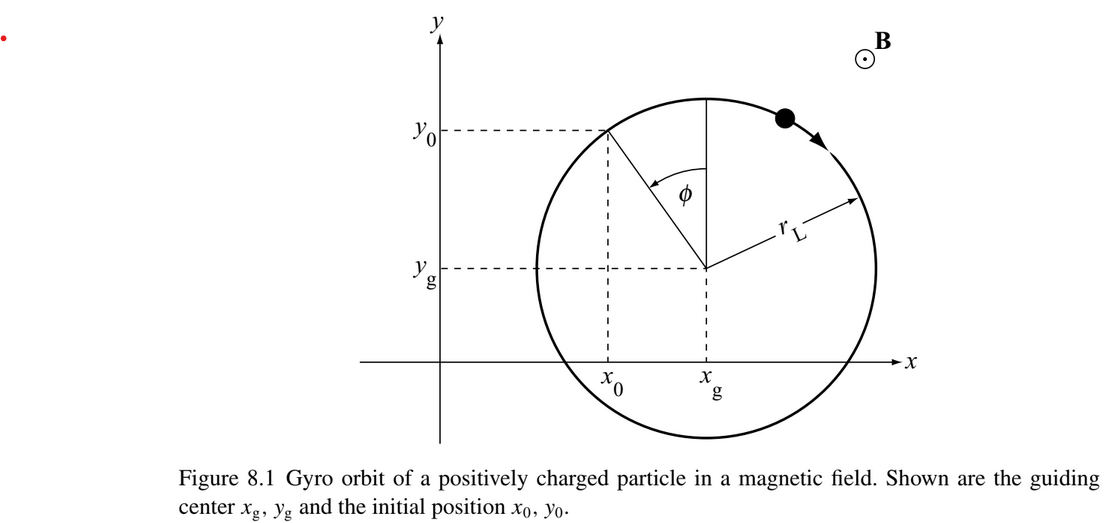
\includegraphics[width=\textwidth]{../../images/gyromotion_coordinates.png}
    \caption{Coordinates for gyromotion (extracted from Plasma Physics and Fusion Energy, J. P. Freidberg).}
    \label{fig:gyromotion_coordiantes}
\end{figure}

\label{sec:only_B_field}
Let's orient our coordinate system such that $\Bvec$ points in the $\evec_z$ direction. Thus, the equations of motion are
\begin{subequations}
\begin{alignat}{2}
    &\frac{d v_x}{dt} = \frac{eB}{m} v_y  \qquad && v_x(0) = v_\perp \cos(\phi), \label{eq:only_B_1} \\
    &\frac{d v_y}{dt} = -\frac{eB}{m} v_x  \qquad && v_y(0) = v_\perp \sin(\phi), \label{eq:only_B_2} \\
    &\frac{d v_z}{dt} = 0  \qquad && v_z(0) = v_{||}. \label{eq:only_B_3}
\end{alignat}
\end{subequations}
The $z$ component is decoupled from the rest and has a trivial solution. For the other two components, we begin by taking the time derivative of \cref{eq:only_B_2}. Thus
\begin{equation}
    \frac{d^2 v_y}{dt^2} = -\frac{eB}{m} \frac{d v_x}{dt} = -w_c^2 v_y,
\end{equation}
where $w_c = |e|B/m$ is the gyro frequency. We know that the general solution to the above is $v_y = c_1 \cos(w_c t) + c_2 \sin(w_c t)$. If we use the ICs and assume ions, we have
\begin{equation}
\label{eq:vel_gyro_y}
    v_y = -v_\perp \sin(w_ct - \phi).
\end{equation}
Integrating \cref{eq:only_B_1} then gives
\begin{equation}
\label{eq:vel_gyro_x}
    v_x = v_\perp \cos(w_c t - \phi).
\end{equation}
The final solution, for either positive or negative charges, can be written as
\begin{align}
\label{eq:vel_gyro}
    v^{(c)}_x &= v_\perp \cos(w_c t \pm \phi) \nonumber \\
    v^{(c)}_y &= \pm v_\perp \sin(w_c t \pm \phi),
\end{align}
where upper signs correspond to a negative charge. Integrating the equations above leads to
\begin{align}
\label{eq:pos_gyro}
    x^{(c)} &= r_L \sin(w_c t \pm \phi) \nonumber \\
    y^{(c)} &= \mp r_L \cos(w_c t \pm \phi).
\end{align}
where $r_L = v_\perp/w_c$ is the gyro radius.

%--------------------------------------------
\subsection{Both $\Evec$ and $\Bvec$ fields}
%--------------------------------------------
\label{sec:E_and_B_field}
Let's orient our coordinate system such that $\Bvec$ still points along $\evec_z$. The equations of motion are
\begin{subequations}
\label{eq:single_particle_motion_EcrossB_temp1}
\begin{alignat}{2}
    &\frac{d v_x}{dt} = \frac{eE_x}{m} + \frac{eB}{m} v_y  \qquad && v_x(0) = v_\perp \cos(\phi) + \frac{E_y}{B}, \label{eq:E_and_B_1} \\
    &\frac{d v_y}{dt} = \frac{eE_y}{m} - \frac{eB}{m} v_x  \qquad && v_y(0) = v_\perp \sin(\phi) - \frac{E_x}{B}, \label{eq:E_and_B_2} \\
    &\frac{d v_z}{dt} = \frac{e E_{||}}{m}  \qquad && v_z(0) = v_{||}, \label{eq:E_and_B_3}
\end{alignat}
\end{subequations}
where we have chosen the given initial conditions simply to facilitate the math. Again, the z component is decoupled from the rest and has the trivial solution $v_z = v_{||} +  (eE_{||}/m) t$. Thus, \cref{eq:single_particle_motion_vel_general} for the $x$ and $y$ components are
\begin{align}
    \label{eq:single_particle_motion_EcrossB_temp2}
    v_x &= v_x^{(c)} + v^{(g)}_x, \nonumber \\
    v_y &= v_y^{(c)} + v^{(g)}_y.
\end{align}
We assume $v^{(g)}_x$ and $v^{(g)}_y$ are time independent. Using \cref{eq:single_particle_motion_EcrossB_temp2} in \cref{eq:single_particle_motion_EcrossB_temp1} we obtain
\begin{align}
    0 &= \frac{eE_x}{m} + \frac{eB}{m}v^{(g)}_y \nonumber \\
    0 &= \frac{eE_y}{m} - \frac{eB}{m}v^{(g)}_x.
\end{align}
Thus, $v^{(g)}_x = E_y/B$ and $v^{(g)}_y = -E_x/B$, which in vector notation can be expressed as
\begin{equation}
    \vvec^{(g)}_E = \frac{\Evec \times \Bvec}{B^2}.
\end{equation}

%-------------------------------------------------------------------------------
\section{Non-uniform $\Bvec$ field}
%-------------------------------------------------------------------------------
%--------------------------------------------
\subsection{Change in magnitude along perpendicular directions}
%--------------------------------------------
The magnetic field still points in the $\evec_z$ direction, but its magnitude changes in directions perpendicular to $\evec_z$: $B = B(q_x,q_y)$. The equations of motion are
\begin{subequations}
\begin{alignat}{2}
    &\frac{d v_x}{dt} = \frac{eB(x,y)}{m} v_y  \qquad && v_x(0) = v_\perp \cos(\phi) -\frac{v^2_\perp}{2 w_c} \left . \frac{\partial B}{\partial q_y} \right |_{x^{(g)},y^{(g)}} \frac{1}{B(x^{(g)},y^{(g)})}, \label{eq:nonuniB_1} \\
    &\frac{d v_y}{dt} = -\frac{eB(x,y)}{m} v_x  \qquad && v_y(0) = v_\perp \sin(\phi) + \frac{v^2_\perp}{2 w_c} \left . \frac{\partial B}{\partial q_x} \right |_{x^{(g)},y^{(g)}} \frac{1}{B(x^{(g)},y^{(g)})}, \label{eq:nonuniB_2} \\
    &\frac{d v_z}{dt} = 0  \qquad && v_z(0) = v_{||}. \label{eq:nonuniB_3}
\end{alignat}
\end{subequations}
In the above, the $x$ and $y$ in $B(x,y)$ are the perpendicular components of the particle's position. The $v_z$ component is decoupled from the rest and has a trivial solution. Thus, \cref{eq:single_particle_motion_vel_general,eq:single_particle_motion_pos_general} for the $x$ and $y$ components are
\begin{equation}
    \label{eq:single_particle_motion_vel_Bmag_change_perp_1}
    v_x = v_x^{(c)} + v_x^{(g)},
\end{equation}
\begin{equation}
    \label{eq:single_particle_motion_vel_Bmag_change_perp_2}
    v_y = v_y^{(c)} + v_y^{(g)},
\end{equation}
\begin{equation}
    \label{eq:single_particle_motion_pos_Bmag_change_perp_1}
    x = x^{(c)} + x^{(g)},
\end{equation}
\begin{equation}
    \label{eq:single_particle_motion_pos_Bmag_change_perp_2}
    y = y^{(c)} + y^{(g)}.
\end{equation}

We begin by employing a Taylor-series expansion for the magnetic field
\begin{equation}
    B(x,y) = B(x^{(g)}, y^{(g)}) + \left . \frac{\partial B}{\partial q_x} \right |_{x^{(g)},y^{(g)}} x^{(c)} + \left . \frac{\partial B}{\partial q_y} \right |_{x^{(g)},y^{(g)}} y^{(c)} + ...
\end{equation}
Thus, \cref{eq:nonuniB_1,eq:nonuniB_2} are now
\begin{equation}
    \frac{ d v_x}{dt} = \frac{e B(x^{(g)},y^{(g)})}{m} v_y + \frac{e}{m} \left ( \left . \frac{\partial B}{\partial q_x} \right|_{x^{(g)},y^{(g)}} x^{(c)} + \left . \frac{\partial B}{\partial q_y} \right |_{x^{(g)},y^{(g)}} y^{(c)} \right) v_y
\end{equation}
\begin{equation}
    \frac{ d v_y}{dt} = -\frac{e B(x^{(g)},y^{(g)})}{m} v_x + \frac{e}{m} \left ( \left . \frac{\partial B}{\partial q_x} \right|_{x^{(g)},y^{(g)}} x^{(c)} + \left . \frac{\partial B}{\partial q_y} \right |_{x^{(g)},y^{(g)}} y^{(c)} \right ) v_x.
\end{equation}
As before, we assume $v_x^{(g)}$, $v_y^{(g)}$ are time independent. Also, for simplicity we assume ions only. Plugging in \cref{eq:single_particle_motion_vel_Bmag_change_perp_1,eq:single_particle_motion_vel_Bmag_change_perp_2} into the above, we get
\begin{equation}
    0 = B(x^{(g)},y^{(g)}) v_y^{(g)} + \left ( \left . \frac{\partial B}{\partial q_x} \right|_{x^{(g)},y^{(g)}} x^{(c)} + \left . \frac{\partial B}{\partial q_y} \right |_{x^{(g)},y^{(g)}} y^{(c)} \right) \left ( v_y^{(c)} + v_y^{(g)} \right),
\end{equation}
\begin{equation}
    0 = -B(x^{(g)},y^{(g)}) v_x^{(g)} + \left ( \left . \frac{\partial B}{\partial q_x} \right|_{x^{(g)},y^{(g)}} x^{(c)} + \left . \frac{\partial B}{\partial q_y} \right |_{x^{(g)},y^{(g)}} y^{(c)} \right ) \left ( v_x^{(c)} + v_x^{(g)} \right ).
\end{equation}
We assume $v_x^{(g)} \ll v_x^{(c)}$ and $v_y^{(g)} \ll v_y^{(c)}$. Thus, the above becomes
\begin{equation}
    \label{eq:single_particle_motion_Bmag_change_perp_temp1}
    0 = B(x^{(g)},y^{(g)}) v_y^{(g)} + \left ( \left . \frac{\partial B}{\partial q_x} \right|_{x^{(g)},y^{(g)}} x^{(c)} + \left . \frac{\partial B}{\partial q_y} \right |_{x^{(g)},y^{(g)}} y^{(c)} \right) v_y^{(c)},
\end{equation}
\begin{equation}
    \label{eq:single_particle_motion_Bmag_change_perp_temp2}
    0 = -B(x^{(g)},y^{(g)}) v_x^{(g)} + \left ( \left . \frac{\partial B}{\partial q_x} \right|_{x^{(g)},y^{(g)}} x^{(c)} + \left . \frac{\partial B}{\partial q_y} \right |_{x^{(g)},y^{(g)}} y^{(c)} \right ) v_x^{(c)}.
\end{equation}
We now use the definitions in \cref{eq:vel_gyro} and \cref{eq:pos_gyro}. For example, with those definitions we can show that 
\begin{align}
     x^{(c)} v_y^{(c)} &= \left[ r_L \sin (w_c t - \phi) \right] \left[ -v_\perp \sin (w_ct - \phi) \right] \nonumber \\
    & = -\frac{ v^2_\perp}{w_c} \sin^2(w_c t - \phi) \nonumber \\
    & = -\frac{ v^2_\perp}{2 w_c} \{1 - \cos [ 2 (w_c t - \phi)] \}
\end{align}
Similar derivations can be carried out for $y^{(c)} v_y^{(c)}$, $x^{(c)} v_x^{(c)}$, and $y^{(c)} v_x^{(c)}$. Thus, \cref{eq:single_particle_motion_Bmag_change_perp_temp1,eq:single_particle_motion_Bmag_change_perp_temp2} become 
\begin{multline}
    0 = B(x^{(g)},y^{(g)}) v_y^{(g)} -\frac{ v^2_\perp}{2 w_c} \left . \frac{\partial B}{\partial q_x} \right |_{x^{(g)},y^{(g)}} \{1 - \cos [ 2 (w_c t - \phi)] \} \\
    - \frac{ v^2_\perp}{2 w_c} \left .\frac{\partial B}{\partial q_y} \right |_{x^{(g)},y^{(g)}} \sin [ 2(w_ct - \phi)],
\end{multline}
\begin{multline}
    0 = -B(x^{(g)},y^{(g)}) v_x^{(g)} -\frac{ v^2_\perp}{2 w_c} \left . \frac{\partial B}{\partial q_x} \right |_{x^{(g)},y^{(g)}} \sin [ 2 (w_c t - \phi)] \\
    - \frac{ v^2_\perp}{2 w_c} \left .\frac{\partial B}{\partial q_y} \right |_{x^{(g)},y^{(g)}} \{ 1 + \cos [ 2(w_ct - \phi)] \}.
\end{multline}
We neglect the oscillatory terms containing the sines and cosines---if it was not possible to neglect them, then the assumption that $v^{(g)}_x$, $v^{(g)}_y$ are time independent would not hold. Thus,
\begin{subequations}
\begin{alignat}{2}
    0 &= B(x^{(g)},y^{(g)}) v_y^{(g)} - \frac{ v^2_\perp}{2 w_c} \left . \frac{\partial B}{\partial q_x} \right |_{x^{(g)},y^{(g)}} \nonumber \\
    0 &= -B(x^{(g)},y^{(g)}) v_x^{(g)} -\frac{ v^2_\perp}{2 w_c} \left . \frac{\partial B}{\partial q_y} \right |_{x^{(g)},y^{(g)}} . 
\end{alignat}
\end{subequations}
Solving for the guiding center velocities, we finally have
\begin{align}
    v_x^{(g)} &= -\frac{v^2_\perp}{2 w_c} \left . \frac{\partial B}{\partial q_y} \right |_{x^{(g)},y^{(g)}} \frac{1}{B(x^{(g)},y^{(g)})} \nonumber \\
    v_y^{(g)} &= \frac{v^2_\perp}{2 w_c} \left . \frac{\partial B}{\partial q_x} \right |_{x^{(g)},y^{(g)}} \frac{1}{B(x^{(g)},y^{(g)})} . 
\end{align}
In vector notation, this is written as
\begin{equation}
    \vvec^{(g)}_{\nabla B} = \mp \frac{v^2_\perp}{2 w_c} \frac{ \Bvec \times \nabla B }{B^2}.
\end{equation}
In the above, the fields and $w_c$ are evaluated at $(x^{(g)},y^{(g)})$.

%--------------------------------------------
\subsection{Change in magnitude along parallel directions}
%--------------------------------------------
Ideally, one would introduce a gradient only in the direction parallel to the magnetic field, that is, one would have $\Bvec = B(q_z) \evec_z$. However, due to Gauss's law, this is too restrictive and instead we generalize and use $\Bvec = B_x \evec_x + B_z \evec_z$, where $B_x = B_x(q_x,q_z)$ and $B_z = B_z(q_x,q_z)$. Thus, the equations of motion are
\begin{align}
    \frac{dv_x}{dt} &= \frac{e}{m} v_y B_z(x,z) , \label{eq:par_grad_vx_inter}\\
    \frac{dv_y}{dt} &= -\frac{e}{m} [v_x B_z(x,z) - v_z B_x(x,z)] , \label{eq:par_grad_vy_inter}\\
    \frac{dv_z}{dt} &= -\frac{e}{m} v_y B_x(x,z) \label{eq:par_grad_vz_inter}.
\end{align}
However, the $z$ direction no longer corresponds to the parallel direction, since the magnetic field also has a component along the $x$ direction. To account for this, we will introduce a rotating reference frame, in which one of the axis will always be aligned with the magnetic field vector, and thus would denote the parallel direction. In the original static reference frame the unit vectors are $(\evec_x, \evec_y, \evec_z)$ and the velocity components are $(v_x, v_y, v_x)$, whereas in this new rotating reference frame the unit vectors are $(\evec_{\perp1}, \evec_{\perp2}, \bvec)$ and the velocity components are $(v_{\perp1}, v_{\perp2}, v_{||})$. 

The rotating reference frame is described by the rotation matrix
\begin{equation}
    \Qvec(t) = \begin{bmatrix} b_x & 0 & b_z \\ 0 & 1 & 0 \\ b_z & 0 & -b_x \end{bmatrix},
\end{equation}
where $b_x = b_x(t)$ and $b_y = b_y(t)$ are given by
\begin{equation}
    b_x = \frac{B_x(x,z)}{B(x,z)} \qquad b_z = \frac{B_z(x,z)}{B(x,z)} \label{eq:bvec_components}
\end{equation}
In the above, $B(x,z) = [ B_x^2(x,z) + B_z^2(x,z) ]^{1/2}$. As an example, the matrix above leads to the following transformations for the unit vectors and velocities in the rotating reference frame 
\begin{align}
    \bvec &= b_x \evec_x + b_z \evec_z \\
    \evec_{\perp2} &= \evec_y \\
    \evec_{\perp1} &= b_z \evec_x - b_x \evec_z = \evec_{\perp2} \times \bvec,
\end{align}
\begin{align}
    v_{||} &= b_x v_x + b_z v_z \label{eq:par_grad_vel_trans_1}\\
    v_{\perp2} &= v_y \label{eq:par_grad_vel_trans_2}\\
    v_{\perp1} &= b_z v_x - b_x v_z. \label{eq:par_grad_vel_trans_3}
\end{align}
Using the transformation rule for the acceleration of a particle, but for some reason neglecting the coriollis and centrifugal forces, we obtain for the velocity derivatives
\begin{align}
    \frac{dv_{||}}{dt} &= \frac{dv_x}{dt} b_x + \frac{dv_z}{dt} b_z  - K v_{\perp1} \\
    \frac{dv_{\perp2}}{dt} &= \frac{dv_y}{dt}\\
    \frac{dv_{\perp1}}{dt} &= \frac{dv_x}{dt} b_z - \frac{dv_z}{dt} b_x + K v_{||},
\end{align}
where $K = K(t)$ is given by $K = b_x db_z/dt - b_z db_x/dt$. Using \cref{eq:par_grad_vx_inter,eq:par_grad_vy_inter,eq:par_grad_vz_inter} in the above leads to
\begin{align}
    \frac{d v_{||}}{dt} &= \frac{e}{m} v_y [B_z(x,z) b_x - B_x(x,z) b_z] - Kv_{\perp1} \\
    \frac{dv_{\perp2}}{dt} &= -\frac{eB}{m} (v_x b_z - v_z b_x) \\
    \frac{dv_{\perp1}}{dt} &= \frac{e}{m} v_y [B_z(x,z) b_z + B_x(x,z) b_x] + Kv_{||} 
\end{align}
Using the definitions for $b_x$ and $b_z$ in \cref{eq:bvec_components}, as well as the expressions for $v_{\perp1}$, $v_{\perp2}$ in \cref{eq:par_grad_vel_trans_2,eq:par_grad_vel_trans_3}, we get
\begin{align}
    \frac{d v_{||}}{dt} &= -Kv_{\perp1}, \label{eq:par_grad_vpar_inter} \\
    \frac{dv_{\perp2}}{dt} &= -w_c v_{\perp1}, \label{eq:par_grad_v2_inter} \\
    \frac{dv_{\perp1}}{dt} &= w_c v_{\perp2} + K v_{||}, \label{eq:par_grad_v1_inter}
\end{align}
where $w_c = w_c(t)$ is given by $w_c = e B(x,z) / m$.

We now introduce a time transformation to simplify the equations above. To do so, we introduce the following variables
\begin{gather}
    \hat{v}_{||} = \hat{v}_{||}(\tau) \qquad \hat{v}_{\perp2} = \hat{v}_{\perp2}(\tau) \qquad \hat{v}_{\perp1} = \hat{v}_{\perp1}(\tau) \\
    \hat{x} = \hat{x}(\tau) \qquad \hat{z} = \hat{z}(\tau)
\end{gather}
such that
\begin{gather}
    v_{||} = \hat{v}_{||}(h(t)) \qquad v_{\perp2} = \hat{v}_{\perp2}(h(t)) \qquad v_{\perp1} = \hat{v}_{\perp1}(h(t)) \\
    x = \hat{x}(h(t)) \qquad z = \hat{z}(h(t)).
\end{gather}
The function $h(t)$ is given by
\begin{equation}
    h(t) = \int_0^t w_c(t') dt'.
\end{equation}
We also show that
\begin{equation}
    b_x = \frac{B_x(x,z)}{B(x,z)} = \frac{B_x(\hat{x}(h(t)),\hat{z}(h(t)))}{B(\hat{x}(h(t)),\hat{z}(h(t)))},
\end{equation}
and thus
\begin{equation}
    \frac{db_x}{dt} = \frac{dh(t)}{dt} \frac{d}{d\tau} \left [ \frac{B_x(\hat{x},\hat{z})}{B(\hat{x},\hat{z})} \right ]_{\tau = h(t)} = w_c \left .\frac{d \hat{b}_x}{d\tau} \right|_{\tau = h(t)},
\end{equation}
where $\hat{b}_x =\hat{b}_x(\tau)$ is given by $\hat{b}_x= B_x(\hat{x},\hat{z}) / B(\hat{x},\hat{z})$. The analogous holds for $b_z$. This allows us to write
\begin{equation}
    K = w_c \left ( \hat{b}_x \frac{d\hat{b}_z}{d \tau} - \hat{b}_z \frac{d\hat{b}_x}{d \tau} \right )_{\tau = h(t)} = w_c \left. \hat{K} \right |_{\tau = h(t)},
\end{equation}
where $\hat{K} = \hat{K}(\tau)$ is given by $\hat{K} = \hat{b}_x d\hat{b}_z/d\tau - \hat{b}_z d\hat{b}_x/d\tau$. With these transformation, \cref{eq:par_grad_vpar_inter,eq:par_grad_v2_inter,eq:par_grad_v1_inter} are re-written as
\begin{align}
    \frac{d\hat{v}_{||}}{d\tau} &= -\hat{K} \hat{v}_{\perp1},\\
    \frac{d\hat{v}_{\perp2}}{d\tau} &= -\hat{v}_{\perp1},\\
    \frac{d\hat{v}_{\perp1}}{d\tau} &= \hat{v}_{\perp2} + \hat{K} \hat{v}_{||}.
\end{align}

We now simplify $B_z$ so that $B_z = B_z(q_z)$. To be consistent with Gauss's law, we require $B_x = B_x(q_x,q_y)$ where $B_x = -q_x dB_z/dq_z$. With these simplified forms, we have
\begin{align}
    \hat{K} &= -\hat{b}_z^2 \frac{d}{d\tau} \left ( \frac{\hat{b}_x}{\hat{b}_z} \right ) \\
    &= -\frac{B_z^2(\hat{z})}{B^2(\hat{x},\hat{z})} \frac{d}{d\tau} \left ( \frac{B_x(\hat{x},\hat{z})}{B_z(\hat{z})} \right ) \\
    &= \frac{B_z^2(\hat{z})}{B^2(\hat{x},\hat{z})} \frac{d}{d\tau} \left [ \hat{x}  \left ( \frac{1}{B_z} \frac{dB_z}{dq_z} \right )_{q_z = \hat{z}} \right ].
\end{align}
We now use the long-thin approximation. For this approximation, we assume that $B_x / B_z \ll 1$, and also that $\frac{1}{B_z} \frac{dB_z}{dq_z}$ changes very slowly. We thus have
\begin{equation}
\label{eq:par_grad_k_inter}
    \hat{K} \approx \frac{d \hat{x}}{d\tau} \left ( \frac{1}{B_z} \frac{dB_z}{dq_z} \right)_{q_z = \hat{z}}.
\end{equation}
Also, using the long-thin approximation in \cref{eq:par_grad_vel_trans_1,eq:par_grad_vel_trans_3} allows us to write
\begin{align}
    v_{||} &\approx v_z = \frac{dz}{dt} = \left ( \frac{d\hat{z}}{d\tau} \right )_{\tau = h(t)} w_c \\
    v_{\perp1} & \approx v_x = \frac{dx}{dt} = \left ( \frac{d \hat{x}}{d\tau} \right )_{\tau = h(t)} w_c.
\end{align}
Evaluating the above at $t = h^{-1}(\tau)$, and defining $\hat{w}_c(\tau)$ from $w_c = \hat{w}_c(h(t))$, we obtain
\begin{align}
    \hat{v}_{||} &\approx  \frac{d\hat{z}}{d\tau}  \hat{w}_c \\
    \hat{v}_{\perp1} & \approx \frac{d \hat{x}}{d\tau} \hat{w}_c.
\end{align}
We also note that
\begin{equation}
    \frac{d B_z(\hat{z})}{d\tau} = \left ( \frac{dB_z}{dq_z} \right )_{q_z = \hat{z}} \frac{d \hat{z}}{d\tau}.
\end{equation}
Using the expressions above in \cref{eq:par_grad_k_inter}, one can approximate $\hat{K}$ using either of the two forms below
\begin{equation}
    \hat{K} \approx \frac{\hat{v}_{\perp1}}{\hat{w}_c B_z(\hat{z})} \left ( \frac{dB_z}{dq_z} \right )_{q_z = \hat{z}} \approx \frac{\hat{v}_{\perp1}}{\hat{v}_{||} B_z(\hat{z})} \frac{dB_z(\hat{z})}{d\tau} .
\end{equation}
We thus write the governing equations for the velocities as
\begin{align}
    \frac{d\hat{v}_{||}}{d\tau} &= -\frac{\hat{v}^2_{\perp1}}{\hat{w}_c B_z(\hat{z})} \left ( \frac{dB_z}{dq_z} \right )_{q_z = \hat{z}} ,\label{eq:par_grad_vpar_thin}\\
    \frac{d\hat{v}_{\perp2}}{d\tau} &= -\hat{v}_{\perp1}, \label{eq:par_grad_v2_thin} \\
    \frac{d\hat{v}_{\perp1}}{d\tau} &= \hat{v}_{\perp2} + \frac{\hat{v}_{\perp1}}{B_z(\hat{z})} \frac{dB_z(\hat{z})}{d\tau}. \label{eq:par_grad_v1_thin}
\end{align}

We now assume the solution for the perpendicular velocities is of the form
\begin{align}
    \hat{v}_{\perp1} &= \hat{v}_\perp \cos [\tau + \hat{\epsilon}] \\
    \hat{v}_{\perp2} &= -\hat{v}_\perp \sin [\tau + \hat{\epsilon}],
\end{align}
where $\hat{v}_\perp = \hat{v}_\perp(\tau)$ and $\hat{\epsilon} = \hat{\epsilon}(\tau)$. Plugging these two assumed solutions into \cref{eq:par_grad_v2_thin,eq:par_grad_v1_thin}, and using some simple algebra, gives
\begin{equation}
    \frac{d\hat{v}_\perp}{d\tau} = \frac{\hat{v}_\perp}{2 B_z(\hat{z})} \frac{dB_z(\hat{z})}{d\tau} \left \{ 1 + \cos [2 (\tau + \hat{\epsilon})] \right \}.
\end{equation}
The above can be re-arranged and expressed as
\begin{equation}
\label{eq:par_grad_mu_evol}
    \frac{d \ln \hat{\mu}}{d\tau} = \frac{d \ln B_z(\hat{z}) }{d\tau} \cos [2 (\tau + \hat{\epsilon})],
\end{equation}
where $\hat{\mu} = \hat{\mu}(\tau)$ is the adiabatic invariant, and is given by
\begin{equation}
    \hat{\mu} = \frac{m \hat{v}^2_\perp}{2 B_z(\hat{z})}.
\end{equation}
Integrating \cref{eq:par_grad_mu_evol} from $\tau_1$ to $\tau_2$ gives
\begin{equation}
    \ln \hat{\mu}(\tau_2) - \ln \hat{\mu}(\tau_1) = \left . \ln [B_z(\hat{z})] \cos [2(\tau + \hat{\epsilon})] \right |^{\tau_2}_{\tau_1} + \int_{\tau_1}^{\tau_2} 2 \ln [ B_z(\hat{z}) ] \sin [2(\tau + \hat{\epsilon})] d\tau.
\end{equation}
Picking $\tau_1$ and $\tau_2$ such that $[\tau_2 + \hat{\epsilon}(\tau_2)] - [\tau_1 + \hat{\epsilon}(\tau_1)] = 2 \pi$, and assuming $B(\hat{z})$ doesn't change significantly from $\tau_1$ to $\tau_2$, gives $\hat{\mu}(\tau_2) = \hat{\mu}(\tau_1)$, that is, $\hat{\mu}$ is constant over one gyro-period. One can also define
\begin{equation}
    \mu = \frac{m v_\perp^2}{2B_z(z)}
\end{equation}
where $\mu = \mu(t)$ and $v_\perp = v_\perp(t)$. Given that $v_\perp = \hat{v}_\perp(h(t))$, we have $\mu = \hat{\mu}(h(t))$. Thus, $\hat{\mu}(\tau_2) = \hat{\mu}(\tau_1)$ translates to $\mu(t_2) = \mu(t_1)$, where $t_2 = h^{-1}(\tau_2)$ and $t_1 = h^{-1}(\tau_1)$.

Finally, we focus not on the perpendicular velocities but the parallel velocity. Plugging-in the assumed solutions in the governing \cref{eq:par_grad_vpar_thin} gives
\begin{equation}
    \frac{d\hat{v}_{||}}{d\tau} = -\frac{\hat{v}^2_{\perp}}{2\hat{w}_c B_z(\hat{z})} \left ( \frac{dB_z}{dq_z} \right )_{q_z = \hat{z}} \{ 1 + \cos [2(\tau + \hat{\epsilon})] \}.
\end{equation}
We now average the above from $\tau_1$ to $\tau_2$ while assuming $B(\hat{z})$, $d\hat{v}_{||}/d\tau$ and $\hat{v}^2_\perp$ do not change significantly during that time scale. Note that since this is an average, we are not just integrating from $\tau_1$ to $\tau_2$, but we are also dividing by $\tau_2 - \tau_1$. After  averaging, we obtain
\begin{equation}
    \frac{d\hat{v}_{||}}{d\tau} = -\frac{\hat{v}^2_{\perp}}{2\hat{w}_c B_z(\hat{z})} \left ( \frac{dB_z}{dq_z} \right )_{q_z = \hat{z}} .
\end{equation}
or
\begin{equation}
    m \frac{d\hat{v}_{||}}{d\tau} = -\frac{\hat{\mu}}{\hat{w}_c} \left ( \frac{dB_z}{dq_z} \right )_{q_z = \hat{z}} .
\end{equation}
Converting back to time $t$ gives
\begin{equation}
    m \frac{dv_{||}}{dt} = -\mu \left ( \frac{dB_z}{dq_z} \right )_{q_z = z} .
\end{equation}


%--------------------------------------------
\subsection{Change in direction}
%--------------------------------------------
Rather than writing \cref{eq:single_particle_motion} in terns if its components as done in previous sections, we leave the equation in vector form. Expressing the velocity as $\vvec = \vvec_\perp + v_{||} \bvec$ and assuming no electric field, we write \cref{eq:single_particle_motion} as
\begin{equation}
    \frac{d}{dt} ( \vvec_\perp + v_{||} \bvec) = \mp w_c (\vvec_\perp + v_{||} \bvec ) \times \bvec,
\end{equation}
where upper sign corresponds to negative charge and lower sign to positive charge. For simplicity we will assume positively charged particles only. We then cross both sides of the above by $\bvec$, that is
\begin{equation}
    \bvec \times \left \{ \left [ \frac{d}{dt} ( \vvec_\perp + v_{||} \bvec) - w_c ( \vvec_\perp + v_{||} \bvec) \times \bvec \right ] \times \bvec \right \} = 0.
\end{equation}
The above is simplified using the following three manipulations
\begin{align}
    \bvec \times \left \{ \left [ w_c ( \vvec_\perp + v_{||} \bvec) \times \bvec \right ] \times \bvec \right \} &= \bvec \times \left \{ \left [ w_c \vvec_\perp \times \bvec \right ] \times \bvec \right \} \nonumber \\
    & = -\bvec \times \left \{ w_c \vvec_\perp ( \bvec \cdot \bvec) - \bvec (\bvec \cdot w_c \vvec_\perp ) \right \} \nonumber \\
    & = w_c \vvec_\perp \times \bvec.
\end{align}
\begin{equation}
    \bvec \times \left \{ \left [ \frac{d\vvec_\perp}{dt} \right ] \times \bvec \right \} = \frac{d \vvec_\perp}{dt}( \bvec \cdot \bvec) - \bvec \left ( \bvec \cdot \frac{d\vvec_\perp}{dt} \right ) = \left ( \frac{d \vvec_\perp}{dt} \right )_\perp.
\end{equation}
\begin{align}
    \bvec \times \left \{ \left [ \frac{d v_{||} \bvec}{dt} \times \bvec \right ] \right \} &= v_{||} \bvec \times \left \{ \left [ \frac{ d\bvec}{dt} \times \bvec \right ] \right \} \nonumber \\
    & = v_{||} \left [ \frac{d \bvec}{dt} ( \bvec \cdot \bvec) - \bvec \left ( \bvec \cdot \frac{d \bvec}{dt} \right ) \right ] \nonumber \\
    & = v_{||} \left [ \frac{d \bvec}{dt} - \bvec \left ( \frac{1}{2} \frac{d \bvec \cdot \bvec}{dt} \right ) \right ] \nonumber \\
    & = v_{||} \frac{d \bvec}{dt}
\end{align}
Thus, we have
\begin{equation}
\label{eq:curvature_1}
    \left ( \frac{ d \vvec_\perp}{dt} \right )_\perp - w_c \vvec_\perp \times \bvec = -v_{||} \frac{d\bvec}{dt}.
\end{equation}
As shown in Freidberg
\begin{equation}
    \frac{d \bvec(\xvec(t))}{dt} = \frac{d \xvec(t)}{dt} \cdot \nabla \bvec = \vvec \cdot \nabla \bvec = \vvec_\perp \cdot \nabla \bvec + v_{||} \bvec \cdot \nabla \bvec,
\end{equation}
where $\nabla \bvec$ is evaluated at $\xvec = \xvec(t)$. Thus, \cref{eq:curvature_1} becomes
\begin{equation}
\label{eq:curvature_2}
    \left ( \frac{ d \vvec_\perp}{dt} \right )_\perp - w_c \vvec_\perp \times \bvec = -v_{||} \vvec_\perp \cdot \nabla \bvec - v_{||}^2 \bvec \cdot \nabla \bvec.
\end{equation}
As was done for the other drifts, we assume the solution is of the form $\vvec_\perp = \vvec^{(c)} + \vvec^{(g)}$, where we assume again that $\vvec^{(g)}$ is time independent. The term $\vvec^{(c)}$ corresponds to gyromotion in a rotating reference frame, and is thus given by 
\begin{equation}
    \vvec^{(c)} = v^{(c)}_{\perp1} \evec_{\perp1} + v^{(c)}_{\perp2} \evec_{\perp2},
\end{equation}
where $\evec_{\perp1}$ and $\evec_{\perp2}$ are orthogonal to $\bvec$ and thus rotate in time. $v^{(c)}_{\perp1}$ is given by \cref{eq:vel_gyro_x} and $v^{(c)}_{\perp2}$ by \cref{eq:vel_gyro_y}. We note that, in the non-rotating reference frame, $\vvec^{(c)}$ is expressed as $\vvec^{(c)} = v^{(c)}_x \evec_x + v^{(c)}_y \evec_y + v^{(c)}_z \evec_z$. We now prove that $\vvec_\perp^{(c)}$ is the solution to the two terms on the left-hand side of \cref{eq:curvature_2}. To show this we first use the transformation rule for the acceleration of a particle in a rotating reference frame, but for some reason ignore the coriollis and centrifugal terms. Thus
\begin{align}
    \frac{d \vvec^{(c)}}{dt} &= \frac{dv^{(c)}_x}{dt} \evec_x + \frac{dv^{(c)}_y}{dt} \evec_y + \frac{dv^{(c)}_z}{dt} \evec_z \nonumber \\ &= \frac{dv^{(c)}_{\perp1}}{dt} \evec_{\perp1} + \frac{dv^{(c)}_{\perp2}}{dt} \evec_{\perp2} + 2\Omega \times \vvec^{(c)}.
\end{align}
We do not allow the rotating reference frame to rotate about the $\bvec$ axis. Thus, $\Omega = \Omega_{\perp1} \evec_{\perp1} + \Omega_{\perp2} \evec_{\perp2}$. Given that $\Omega$ and $\vvec^{(c)}$ are in the same plane, $\Omega \times \vvec^{(c)}$ must point in the $\bvec$ direction. Thus, 
\begin{equation}
    \left ( \frac{d \vvec^{(c)}}{dt} \right )_\perp = \frac{dv^{(c)}_{\perp1}}{dt} \evec_{\perp1} + \frac{dv^{(c)}_{\perp2}}{dt} \evec_{\perp2}.
\end{equation}
This allows us to show that 
\begin{equation}
    \left ( \frac{d \vvec^{(c)}}{dt} \right )_\perp - w_c \vvec^{(c)} \times \bvec = \frac{dv^{(c)}_{\perp1}}{dt} \evec_{\perp1} + \frac{dv^{(c)}_{\perp2}}{dt} \evec_{\perp2} - w_c v^{(c)}_{\perp2} \evec_{\perp1} + w_c v^{(c)}_{\perp1} \evec_{\perp2} = 0.
\end{equation}
We now plug in $\vvec_\perp = \vvec^{(c)} + \vvec^{(g)}$ in \cref{eq:curvature_2} to obtain
\begin{equation}
\label{eq:curvature_3}
    -w_c \vvec^{(g)} \times \bvec = - v_{||} \vvec_\perp \cdot \nabla \bvec - v_{||}^2 \bvec \cdot \nabla \bvec.
\end{equation}
As explained in Freidberg, the term $v_{||} \vvec_\perp \cdot \nabla \bvec$ leads to small modifications of the gyro motion, but does not lead to a drift of the particles, and thus is ignored. Taking the cross product of \cref{eq:curvature_3} with $\bvec$ finally gives the curvature drift
\begin{equation}
    \vvec^{(g)}_\kappa = \pm \frac{v_{||}^2}{w_c} \frac{( \bvec \cdot \nabla \bvec ) \times \Bvec}{B}.
\end{equation}

We now show that, if we assume $\nabla \times \Bvec = 0$, the grad-B drift 
\begin{equation}
    \vvec^{(g)}_{\nabla B} = \mp \frac{v^2_\perp}{2 w_c} \frac{\Bvec \times \nabla B}{B^2}
\end{equation}
can be written in the same form as the curvature drift. We begin by showing that
\begin{equation}
    \Bvec \times \nabla B = \Bvec \times \nabla \left ( \Bvec \cdot \Bvec \right )^{1/2} = \Bvec \times \frac{1}{2B} \nabla \left ( \Bvec \cdot \Bvec \right ).
\end{equation}
We now use the vector identity $\nabla (\Bvec \cdot \Bvec ) = 2 \Bvec \times (\nabla \times \Bvec) + 2 \Bvec \cdot \nabla \Bvec$, and assume magnetic curl of zero to obtain
\begin{align}
    \Bvec \times \nabla B &= \Bvec \times \frac{1}{B} \Bvec \cdot \nabla \Bvec \nonumber \\
    &= \Bvec \times \bvec \cdot \nabla (B \bvec) \nonumber \\
    &= \Bvec \times \left (\bvec \cdot \nabla B \right ) \bvec + \Bvec \times B \left (\bvec \cdot \nabla \bvec \right ) \nonumber \\
    &= -B \left ( \bvec \cdot \nabla \bvec \right ) \times \Bvec.
\end{align}
Thus, the grab-B drift can be written as 
\begin{equation}
    \vvec^{(g)}_{\nabla B} = \pm \frac{v^2_\perp}{2 w_c} \frac{(\bvec \cdot \nabla \bvec) \times \Bvec}{B}.
\end{equation}

%-------------------------------------------------------------------------------
\section{Non-uniform $\Evec$ field}
%-------------------------------------------------------------------------------

%-------------------------------------------------------------------------------
\section{Time-varying $\Evec$ field}
%-------------------------------------------------------------------------------
Consider the scenario used in \cref{sec:E_and_B_field}, but with a time varying electric field. The equations of motion are
\begin{subequations}
\label{eq:time_var_E_temp1}
\begin{alignat}{2}
    &\frac{d v_x}{dt} = \frac{eE_x(t)}{m} + \frac{eB}{m} v_y  \qquad && v_x(0) = v_\perp \cos(\phi) + \frac{E_y(t)}{B} + \frac{m}{eB^2}\frac{dE_x(t)}{dt},  \\
    &\frac{d v_y}{dt} = \frac{eE_y(t)}{m} - \frac{eB}{m} v_x  \qquad && v_y(0) = v_\perp \sin(\phi) - \frac{E_x(t)}{B} + \frac{m}{eB^2}\frac{dE_y(t)}{dt},  \\
    &\frac{d v_z}{dt} = \frac{e E_{||}(t)}{m}  \qquad && v_z(0) = v_{||}, 
\end{alignat}
\end{subequations}
where again we chose the initial conditions simply to be consistent with the solution that we'll derive. The parallel velocity is independent of the perpendicular velocities, and we won't worry about it for now. To solve for the perpendicular velocities, we again assume the general solution is 
\begin{align}
\label{eq:time_var_temp2}
    v_x = v_x^{(c)} + v_x^{(g)} \nonumber \\
    v_y = v_y^{(c)} + v_y^{(g)} 
\end{align}
but now do not assume $v_x^{(g)}$ and $v_y^{(g)}$ are time independent. We expand $v_i^{(g)}$ as 
\begin{equation}
    v_i^{(g)} = v^{(g,1)}_i +  v^{(g,2)}_i + ...,
\end{equation}
where $v_i^{(g,\alpha)} \sim \epsilon v_i^{(g,\alpha-1)}$, and the small parameter $\epsilon$ follows from assuming 
\begin{equation}
\label{eq:time_var_E_temp3}
    \frac{1}{v^{(g,\alpha)}_i} \frac{d v^{(g,\alpha)}_i}{dt} \sim \epsilon w_c.
\end{equation}
That is, the time scale associated with the rate of change of all of the $v^{(g,\alpha)}_i$ components is much larger than the time scale of the gyromotion. In other words, we assume particles gyrate faster than how quickly their drift velocity changes. Using \cref{eq:time_var_temp2} in \cref{eq:time_var_E_temp1} leads to
\begin{align}
    \frac{dv_x^{(g,1)}}{dt} + \frac{dv_x^{(g,2)}}{dt} &= \frac{e E_x(t)}{m} + \frac{eB}{m} v_y^{(g,1)} + \frac{eB}{m} v_y^{(g,2)} \nonumber \\
    \frac{dv_y^{(g,1)}}{dt} + \frac{dv_y^{(g,2)}}{dt} &= \frac{e E_y(t)}{m} - \frac{eB}{m} v_x^{(g,1)} - \frac{eB}{m} v_x^{(g,2)}.
\end{align}
Collecting lowest order terms
\begin{align}
    0 &= \frac{eE_x(t)}{m} + \frac{eB}{m} v_y^{(g,1)}  \nonumber \\
    0 &= \frac{eE_y(t)}{m} - \frac{eB}{m} v_x^{(g,1)} ,
\end{align}
and thus $v^{(g,1)}_x = E_y(t) / B$ and $v^{(g,1)}_y = -E_x(t) / B$, which in vector notation is
\begin{equation}
    \vvec^{(g,1)} = \frac{\Evec(t) \times \Bvec}{B^2}.
\end{equation}
Collecting first order terms 
\begin{align}
    \frac{dv_x^{(g,1)}}{dt} &= \frac{eB}{m} v_y^{(g,2)} \nonumber \\
    \frac{dv_y^{(g,1)}}{dt} &= -\frac{eB}{m} v_x^{(g,2)},
\end{align}
and thus $v_x^{(g,2)} = (m/eB^2)dE_x(t)/dt$ and $v_y^{(g,2)} = (m/eB^2) dE_y(t)/dt$, which in vector notation is
\begin{equation}
    \label{eq:particle_polarization_drift}
    \vvec^{(g,2)} = \mp \frac{1}{w_c B}\frac{d\Evec_\perp}{dt}.
\end{equation}
We note that, by looking at the solutions for $v_x^{(g,1)}$ and $v_y^{(g,1)}$, the assumption in \cref{eq:time_var_E_temp3} is equivalent to stating that the electric field changes slowly. 

%-------------------------------------------------------------------------------
\section{Time-varying $\Bvec$ field}
%-------------------------------------------------------------------------------
Let's assume the magnetic field points in the $z$ direction again. Using Faraday's law, we have
\begin{equation}
    \left(\frac{\partial E_z}{\partial q_y} - \frac{\partial E_y}{\partial q_z} \right) \evec_x - \left(\frac{\partial E_z}{\partial q_x} - \frac{\partial E_x}{\partial q_z} \right) \evec_y + \left(\frac{\partial E_y}{\partial q_x} - \frac{\partial E_x}{\partial q_y} \right) \evec_z = -\frac{\partial B}{\partial t} \evec_z.
\end{equation}
To satisfy the above, we set $E_z = 0$, and $E_x = E_x(q_x,q_y,t)$, $E_y = E_y(q_x,q_y,t)$. That is, a time varying magnetic field requires a time and spatially varying electric field. 

We will further simplify our analysis by having $E_x = 0$ and $E_y = E_y(q_x,t)$. Thus, the equations of motion are
\begin{align}
    \frac{dv_x}{dt} &= \frac{eB(t)}{m} v_y, \\
    \frac{dv_y}{dt} &= \frac{eE_y(x,t)}{m} - \frac{eB(t)}{m}v_x,
\end{align}
with $v_z$ constant. As done in previous sections, the velocities and positions are decomposed as follows
\begin{equation}
    v_x = v_x^{(c)} + v_x^{(g)},
\end{equation}
\begin{equation}
    v_y = v_y^{(c)} + v_y^{(g)},
\end{equation}
\begin{equation}
    x = x^{(c)} + x^{(g)},
\end{equation}
\begin{equation}
    y = y^{(c)} + y^{(g)}.
\end{equation}
The electric field is then linearized using a Taylor-series expansion about the guiding center,
\begin{align}
    \frac{dv_x}{dt} &= \frac{eB(t)}{m} v_y \\
    \frac{dv_y}{dt} &= \frac{e}{m} \left [ E_y \left ( x^{(g)},t \right ) + \left .\frac{\partial E_y}{\partial q_x} \right |_{x^{(g)}} x^{(c)} \right ] - \frac{eB(t)}{m}v_x,
\end{align}
We assume positive ions for simplicity and re-write the above as
\begin{align}
    \frac{dv_x}{dt} &= w_c v_y \\
    \frac{dv_y}{dt} &= \frac{w_c}{B(t)} \left [ E_y \left ( x^{(g)},t \right ) + \left .\frac{\partial E_y}{\partial q_x} \right |_{x^{(g)}} x^{(c)} \right ] - w_c v_x.
\end{align}
where $w_c = w_c(t)$. We introduce new variables 
\begin{gather}
    \hat{v}_x = \hat{v}_x(\tau) \qquad \hat{v}_y = \hat{v}_y(\tau) \qquad \hat{x}^{(c)} = \hat{x}^{(c)}(\tau) \qquad \hat{x}^{(g)} = \hat{x}^{(g)}(\tau) \nonumber \\ \hat{E}_y = \hat{E}_y(q_x,\tau) \qquad \hat{B} = \hat{B}(\tau)
\end{gather}
such that 
\begin{gather}
    v_x(t) = \hat{v}_x(h(t)) \qquad
    v_y(t) = \hat{v}_y(h(t)) \qquad
    x^{(c)}(t) = \hat{x}^{(c)}(h(t)) \quad
    x^{(g)}(t) = \hat{x}^{(g)}(h(t)) \nonumber \\
    E_y(q_x,t) = \hat{E}_y(q_x,h(t)) \qquad
    B(t) = \hat{B}(h(t)).
\end{gather}
For the above
\begin{equation}
    h(t) = \int_0^t w_c(t') \, dt'.
\end{equation}
The equations of motion then become
\begin{align}
\label{eq:time_var_B_inter_1}
    \frac{d \hat{v}_x}{d \tau} &= \hat{v}_y \nonumber \\
    \frac{d \hat{v}_y}{d \tau} &= \frac{1}{\hat{B}(\tau)} \left [ \hat{E}_y(\hat{x}^{(g)},\tau) + \left .\frac{\partial \hat{E}_y}{\partial q_x} \right |_{\hat{x}^{(g)}} \hat{x}^{(c)} \right ] - \hat{v}_x.
\end{align}

For the gyromotion quantities, we'll assume they are of the following form,
\begin{align}
    \hat{v}_x^{(c)} &= \hat{v}_\perp \cos(\tau + \hat{\epsilon}), \\
    \hat{v}_y^{(c)} &= -\hat{v}_\perp \sin(\tau + \hat{\epsilon}), \\
    \hat{x}^{(c)} &= \hat{r}_L \sin(\tau + \hat{\epsilon}), \\
    \hat{y}^{(c)} &= \hat{r}_L \cos(\tau + \hat{\epsilon}),
\end{align} 
where $\hat{v}_\perp = \hat{v}_\perp(\tau)$, $\hat{\epsilon} = \hat{\epsilon}(\tau)$, $\hat{w}_c = \hat{w}_c(\tau) = e \hat{B}(\tau)/m$, and $\hat{r}_L = \hat{v}_\perp / \hat{w}_c$ are now time-dependent functions. Note that for this specific case, the $\tau$-derivatives of the positions above are not equal to their respective velocities, and instead the relationship holds only to leading order. For the guiding center velocities, we'll guess a given form and then check if it satisfies the governing equations. Thus, we guess
\begin{align}
    \hat{v}_x^{(g)} &= \frac{\hat{E}_y(\hat{x}^{(g)},\tau)}{\hat{B}(\tau)} \nonumber \\
    \hat{v}_y^{(g)} &= \frac{d}{d \tau} \left ( \frac{\hat{E}_y(\hat{x}^{(g)},\tau)}{\hat{B}(\tau)} \right ).
\end{align}

Plugging in all of these expressions in the evolution equations given by \cref{eq:time_var_B_inter_1}, and using a bit of algebra, leads to
\begin{equation}
\frac{d \ln \hat{\mu}}{d\tau} = \frac{d \ln \hat{B}(\tau)}{d\tau} \cos [ 2 (\tau + \hat{\epsilon}) ],
\end{equation}
where $\hat{\mu} = \hat{\mu}(\tau)$ is given by
\begin{equation}
    \hat{\mu} = \frac{m \hat{v}_\perp^2}{2\hat{B}(\tau)}.
\end{equation}
Integrating over one gyro-period, i.e.\@ from $\tau_1$ to $\tau_2$ such that $[\tau_2 + \epsilon(\tau_2)] - [\tau_1 + \epsilon(\tau_1)] = 2\pi$, gives
\begin{equation}
    \ln \hat{\mu}(\tau_2) - \ln \hat{\mu}(\tau_1) = \left. \ln [\hat{B}(\tau)] \cos [2 (\tau+\hat{\epsilon})] \right |_{\tau_1}^{\tau_2} + \int_{\tau_1}^{\tau_2} 2 \ln [\hat{B}(\tau)] \sin[2(\tau+\hat{\epsilon})] \, d\tau.
\end{equation}
Assuming $\hat{B}(\tau)$ doesn't change significantly from $\tau_1$ to $\tau_2$, then we have $\hat{\mu}(\tau_2) = \hat{\mu}(\tau_1)$, that is, $\hat{\mu}$ is constant over one gyro-period. On can also define
\begin{equation}
    \mu = \frac{m v_\perp^2}{2 B(t)}
\end{equation}
where $\mu = \mu(t)$ and $v_\perp = v_\perp(t)$. Given that $v_\perp = \hat{v}_\perp(h(t))$, we have $\mu = \hat{\mu}(h(t))$. Thus, $\hat{\mu}(\tau_2) = \hat{\mu}(\tau_1)$ translates to $\mu(t_2) = \mu(t_1)$, where $t_2 = h^{-1}(\tau_2)$ and $t_1 = h^{-1}(\tau_1)$.

As shown in the analysis above, for a time dependent magnetic field a drift of the following form is introduced
\begin{equation}
    \hat{v}^{(g)}_y = \frac{d}{d\tau} \left ( \frac{\hat{E}_y(\hat{x}^{(g)},\tau)}{\hat{B}(\tau)} \right ).
\end{equation}
Converting back to time $t$
\begin{equation}
    v^{(g)}_y = \frac{1}{w_c} \frac{d}{dt} \left ( \frac{E_y(x^{(g)},t)}{B(t)} \right ).
\end{equation}
For the more general case where $E_x = E_x(q_x,q_y,t)$ and $E_y = E_y(q_x,q_y,t)$ then
\begin{equation}
    \vvec^{(g)}_p = \mp \frac{1}{w_c} \frac{d}{dt} \left ( \frac{\Evec_\perp}{B} \right ),
\end{equation}
where top sign is for electrons and bottom sign is for ions, and it is assumed that the electric field is evaluated at the guiding center. For an even more general case where the magnetic field does not necessarily point in one direction,
\begin{equation}
    \vvec^{(g)}_p = \mp \frac{1}{w_c} \bvec \times \frac{d\vvec^{(g)}_E}{dt}.
\end{equation}

%--------------------------------------------------------------------------------------------------------------------------------------------
\chapter{Plasma parameters, time scales, and length scales}
%--------------------------------------------------------------------------------------------------------------------------------------------
A summary of fundamental time and length scales of plasmas in given in \cref{tb:plasma_time_scales,tb:plasma_length_scales}
\begin{table}[H]
\renewcommand{\arraystretch}{2.5}
\centering
\caption{Plasma time scales, for either electrons ($\alpha = e$) or ions ($\alpha = i$). }
\label{tb:plasma_time_scales}
 \begin{tabular}{l|l}
    Time scales & Formulas \\
    \hline
    Gyro period  & $\tau_{c\alpha} = \dfrac{2\pi}{w_{c\alpha}} \quad w_{c\alpha} = \dfrac{q_\alpha B}{m_\alpha}$ \\
    Plasma period & $\tau_{p\alpha} = \dfrac{2 \pi }{w_{p\alpha}} \quad w_{p\alpha} = \sqrt{\dfrac{n_\alpha q_\alpha^2}{m_\alpha \epsilon_0}}$
 \end{tabular}
\end{table}

\begin{table}[H]
\renewcommand{\arraystretch}{2.5}
\centering
\caption{Plasma length scales, for either electrons ($\alpha = e$) or ions ($\alpha = i$).}
\label{tb:plasma_length_scales}
 \begin{tabular}{l|l}
   Length scales & Formulas \\
   \hline
   Gyro radius  & $r_{c\alpha} = \dfrac{v_{T\alpha}}{w_{c\alpha}} = \dfrac{m v_{T\alpha}}{q_\alpha B}$ \\
   Debye length & $\lambda_{D\alpha} = \dfrac{v_{T\alpha}}{\sqrt{2} w_{p\alpha}} = \sqrt{ \dfrac{\epsilon_0 k_B T_\alpha}{ n_\alpha q_\alpha^2}}$ \\
   DeBroglie wave length & $\lambda_{B\alpha} = \dfrac{h}{\sqrt{\pi} m_\alpha v_{T\alpha}}$ \\
   Sphere radius & $a_\alpha = \left ( \dfrac{3}{4 \pi n_\alpha} \right )^{1/3}$
\end{tabular}
\end{table}

\begin{itemize}
\item Thermal velocity:
\begin{equation}
v_{T_\alpha} = \sqrt{\frac{2 k_B T_\alpha}{m_\alpha}}
\end{equation}

\item Total Debye length:
\begin{equation}
    \frac{1}{\lambda_D^2} = \sum_\alpha \frac{1}{\lambda_{D\alpha}^2}.
\end{equation}

\item Plasma parameter
\begin{equation}
    \Lambda_\alpha = \frac{4}{3} \pi \lambda_{D\alpha}^3 n_\alpha
\end{equation}

\item Quantum plasma parameter
\begin{equation}
    \chi_\alpha = \frac{4}{3} \pi \lambda_{B\alpha}^3 n_\alpha
\end{equation}

\item Coupling parameter:
\begin{equation}
    \label{eq:def_coupling_parameter}
    \Gamma_\alpha = \frac{q_\alpha^2}{4 \pi \epsilon_0 a_\alpha k_B T_\alpha} = \frac{1}{3} \Lambda_\alpha^{-2/3}
\end{equation}

\item Degeneracy parameter for electrons:
\begin{equation}
    \Theta_e = \frac{k_B T_e}{E_{fe}} = \left( \frac{2^{10} \pi}{3^4} \right)^{1/3} \chi_e^{-2/3}
\end{equation}

\item Fermi energy for electrons:
\begin{equation}
    E_{fe} = \frac{\hbar^2}{2m_e} \left ( 3 \pi^2 n_e \right)^{2/3}
\end{equation}
\end{itemize}

\paragraph{Some notes on the coupling parameter}
We can define two types of Coulomb interactions: strong and weak. Strong Coulomb interactions are those for which the particle's Coulomb potential energy is larger than its kinetic energy, and viceversa for weak Coulomb interactions. Thus, we can also define two types of plasma regimes:
\begin{itemize}
    \item Strongly-coupled plasmas: plasmas where the Coulomb interactions are mostly strong and thus drive the dynamics of its evolution. Coulomb interactions tend to be strong when the inter-particle distances are small, and thus this regime would be dominated by \textit{short-range} interactions. These plasmas are also described as exhibiting \textit{collisional} behavior, since a strong Coulomb interaction essentially means a collision has occurred.
    \item Weakly-coupled plasmas: plasmas where the Coulomb interactions are mostly weak, and as a result do not drive the dynamics of its evolution. The plasma dynamics are instead driven by \textit{long-range} effects caused by smooth electromagnetic fields that result from integrating a large number of particles. These plasmas are also described as exhibiting \textit{collective} behavior, since the long-range electromagnetic fields follow from the collective integration of many particles.
\end{itemize}

We describe an approximate Coulomb potential energy for particles in a plasma as
\begin{equation}
    \text{U} =  \frac{q_\alpha^2}{4 \pi \epsilon_0 a_\alpha}.
\end{equation}
The impact parameter that has been used above is $a_\alpha$, the sphere radius. This provides a decent measure on the average spacing between particles in a plasma. Since the volume of a single particle is $1/n_\alpha$, and if we assume that this volume is given by $4/3 \pi a_\alpha^3$, then equating these two gives the expression for the sphere radius
\begin{equation}
    a_\alpha = \left ( \frac{3}{4 \pi n_\alpha} \right )^{1/3}.
\end{equation}
The kinetic energy of a particle in a plasma can be approximated by the thermal energy, thus
\begin{equation}
    \text{K} = \frac{1}{2} m_\alpha v_{T_\alpha}^2 = k_b T_\alpha.
\end{equation}
The ratio of the particle's Coulomb potential energy and its kinetic energy is referred to as the coupling parameter $\Gamma_\alpha$. That is 
\begin{equation}
    \Gamma_\alpha = \frac{q_\alpha^2}{4 \pi \epsilon_0 a_\alpha k_b T_\alpha}.
\end{equation}
$\Gamma_\alpha > 1$ denotes a strongly coupled plasma, and $\Gamma_\alpha < 1$ denotes a weakly coupled plasma. 

As shown in \cref{eq:def_coupling_parameter}, the coupling and plasma parameters are inversely proportional to each other. Thus, $\Lambda_\alpha < 1$ implies strongly-coupled plasmas, and $\Lambda_\alpha > 1$ weakly-coupled plasmas. Since $\Lambda_\alpha$ represents the number of particles per Debye sphere, it is interesting to note that a large number of particles within such a sphere is needed to be in the weakly-coupled-plasma regime. However, this does not correspond to a plasma with large density, in fact, it corresponds to the opposite. The explicit $n_\alpha$ term in the definition $\Lambda_\alpha = (4/3) \pi \lambda^3_{D\alpha} n_\alpha$ is dominated by the $n_\alpha$ in the denominator of $\lambda_{D\alpha}$. In other words, low plasma densities lead to large Debye spheres, which in turn leads to many particles per Debye sphere, and hence a weakly-coupled plasma.

%--------------------------------------------------------------------------------------------------------------------------------------------
\chapter{Single-particle motion---Collisions}
%--------------------------------------------------------------------------------------------------------------------------------------------
%-------------------------------------------------------------------------------
\section{Cross section}
%-------------------------------------------------------------------------------
The cross section characterizes in a quantitative form the probability that two particles traveling towards each other will undergo an interaction (also sometimes referred to as a collision). For example, imagine an incident particle traveling towards a target particle. This target particle has a spherical force field, and it affects incident particles that come within this sphere. Projecting the spherical force field to a plane perpendicular to the velocity of the incident particle gives a circular cross section. If the incident particle path takes it within this cross section, then the incident particle feels the force field of the target particle, that is, they interact. If the incident particle path does not take it within the cross section, then the particles do not interact. This is an example of a finite cross section, there can also be infinite cross sections for which particles always interact, although the farther away they are the weaker the interaction (e.g. electromagnetic force fields).

\begin{figure}[ht]
\centering
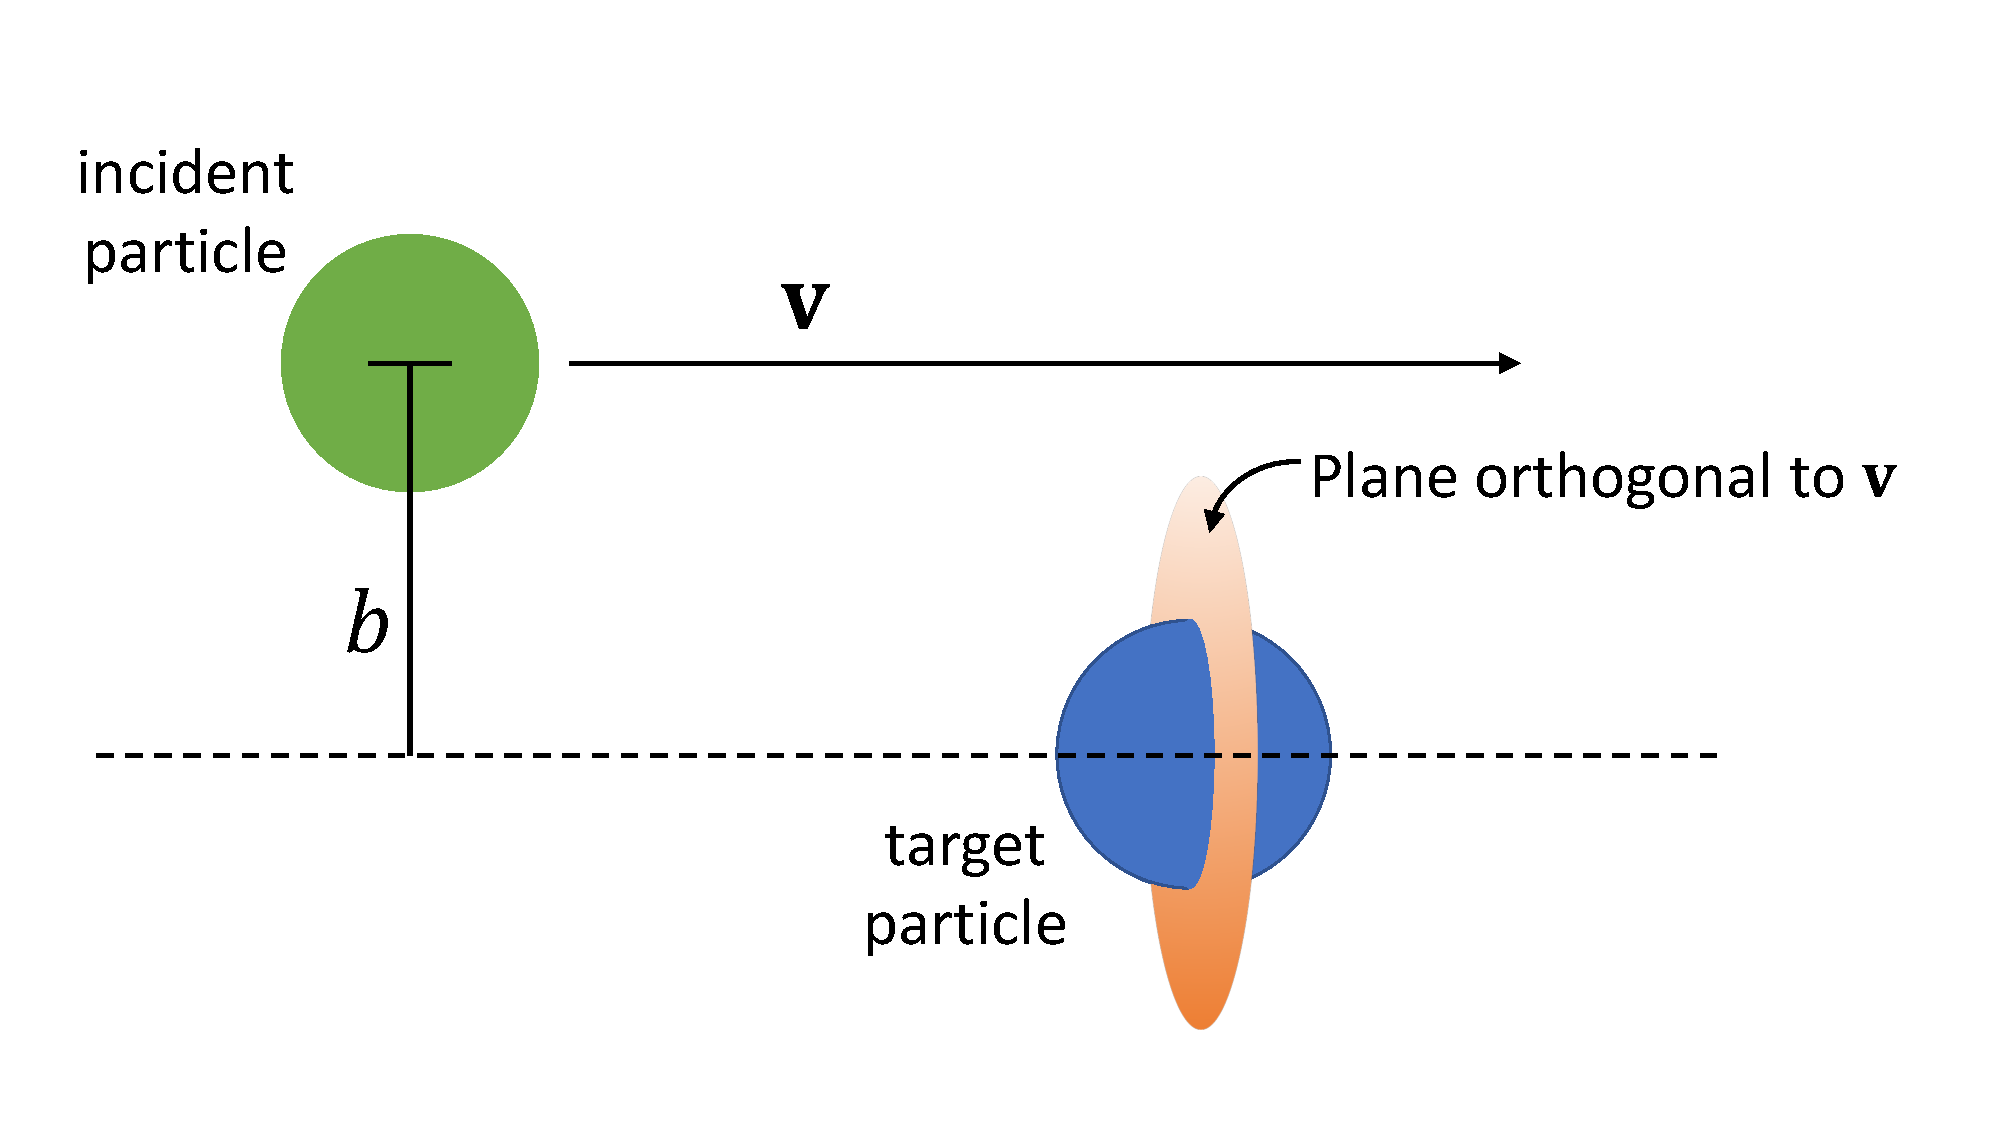
\includegraphics[width=10cm]{../../images/cross_section.pdf}
\caption{Cross section for particle interactions.}
\label{fig:cross_section}
\end{figure}

To quantify the above, the reader is referred to \cref{fig:cross_section}. Imagine an incident particle traveling towards a stationary target particle with an impact parameter $b$ and velocity $\vvec$ (if the target particle is not stationary, then $\vvec = \vvec_2 - \vvec_1$, where $\vvec_1$ is the velocity of the target particle and $\vvec_2$ is the velocity of the incident particle.) As shown in \cref{fig:cross_section}, the impact parameter is the perpendicular offset between the path of the incident particle, and the line parallel to the incident particle velocity that crosses the origin of the target particle (or the origin of the force field of the target particle). To determine the cross section, we ask the following question: for a particle with impact parameter $b$ and velocity magnitude $v = |\vvec|$, does it interact with the target particle? Let's say it does not interact, then the infinitesimal surface located at $b$, i.e.\@ $b db d\phi$ for cylindrical coordinates, does not contribute to the cross section. If it does interact, then $b db d\phi$ does contribute to the cross section. To obtain the total cross section $\sigma = \sigma(v)$, we sum over all infinitesimal areas $b db d\phi$, but account whether a particle at a given $b$ interacts or not with the target particle. This is expressed mathematically as
\begin{equation}
\label{eq:def_cross_section}
    \sigma = \int_0^{2\pi} \int_0^\infty F(v,b) \, b db d\phi.
\end{equation}
In the above $F(v,b) = 1$ if an incident particle with impact parameter $b$ and velocity $v$ interacts with the target particle, and $F(v,b) = 0$ if it does not. However, in reality, $F(v,b)$ is not necessarily binary, and can take other values besides 0 and 1.

An example of $F(v,b)$ is that corresponding to particles that are hard spheres with radius R. For this case, $F(v,b) = H(2R - b)$, where $H$ is the heaviside function. Thus,
\begin{equation}
    \sigma = \int_0^{2\pi} \int_0^\infty H(2R-b) \, b db d\phi = 2\pi \int_0^{2R} b db = \pi (2R)^2,
\end{equation}
as expected.

%-------------------------------------------------------------------------------
\section{Mean free path, collision time, and collision frequency}
%-------------------------------------------------------------------------------
The cross section then defines the mean free path $\lambda_m$, collision time $\tau_m$ and collision frequency $\nu_m$. These are given by
\begin{equation}
    \lambda_m = \frac{1}{n_1 \sigma},
\end{equation}
\begin{equation}
    \tau_m = \frac{\lambda_m}{v} = \frac{1}{n_1 \sigma v},
\end{equation}
and
\begin{equation}
    \nu_{m} = \frac{1}{\tau_m} = n_1 \sigma v.
\end{equation}

%--------------------------------------------------------------------------
\section{Coulomb scattering}
%--------------------------------------------------------------------------
%--------------------------------------------
\subsection{Particle equations}
%--------------------------------------------
Consider two particles, with positions $\rvec_1=\rvec_1(t)$ and $\rvec_2=\rvec_2(t)$, velocities $\vvec_1=\vvec_1(t)$ and $\vvec_2=\vvec_2(t)$, charges $q_1$ and $q_2$, and masses $m_1$ and $m_2$, respectively. Their positions and velocities are governed by the following equations 
\begin{equation}
    \label{eq:particle_1_pos}
    \frac{d \rvec_1}{dt} = \vvec_1,
\end{equation}
\begin{equation}
    \label{eq:particle_2_pos}
    \frac{d \rvec_2}{dt} = \vvec_2,
\end{equation}
\begin{equation}
    \label{eq:particle_1_vel}
    m_1 \frac{d\vvec_1}{dt} = -\frac{q_1 q_2}{4 \pi \epsilon} \frac{\rvec_2 - \rvec_1}{\left | \rvec_2 - \rvec_1 \right |^3},
\end{equation}
\begin{equation}
    \label{eq:particle_2_vel}
    m_2 \frac{d\vvec_2}{dt} = -\frac{q_1 q_2}{4 \pi \epsilon} \frac{\rvec_1 - \rvec_2}{\left | \rvec_1 - \rvec_2 \right |^3}.
\end{equation}
We note that the above system consists of twelve equations for twelve unknowns. We now introduce the center-of-mass position $\Rvec = \Rvec(t)$, the center-of-mass velocity $\Vvec = \Vvec(t)$, the shifted position $\rvec = \rvec(t)$ and the shifted velocity $\vvec = \vvec(t)$ as follows
\begin{equation}
    \Rvec = \frac{m_1 \rvec_1 + m_2 \rvec_2}{m_1 + m_2} \qquad \rvec = \rvec_1 - \rvec_2,
\end{equation}
\begin{equation}
    \Vvec = \frac{m_1 \vvec_1 + m_2 \vvec_2}{m_1 + m_2} \qquad \vvec = \vvec_1 - \vvec_2
\end{equation}
Thus, in terms of these new four variables, the particle equations can be written as
\begin{equation}
    \frac{d \Rvec}{dt} = \Vvec,
\end{equation}
\begin{equation}
    \frac{d \Vvec}{dt} = 0 ,
\end{equation}
\begin{equation}
    \label{eq:particle_pos}
    \frac{d \rvec}{dt} = \vvec,
\end{equation}
\begin{equation}
    \label{eq:particle_vel}
    \frac{d \vvec}{dt} = \frac{q_1 q_2}{4\pi \epsilon_0 m_r} \frac{\rvec}{r^3},
\end{equation}
where the reduced mass $m_r$ is given by
\begin{equation}
    \frac{1}{m_r} = \frac{1}{m_1} + \frac{1}{m_2}.
\end{equation}
The first two equations above give the trivial solution $\Vvec = $ constant and $\Rvec$ = $\Rvec(0) + \Vvec t$. Thus, we have reduced the problem from twelve unknowns to six unknowns, namely $\rvec$ and $\vvec$.

%--------------------------------------------
\subsection{Conservation of energy}
%--------------------------------------------
Dotting \cref{eq:particle_vel} by $\vvec$ gives 
\begin{align}
    \vvec \cdot \frac{d \vvec}{dt} &= \frac{q_1 q_2}{4 \pi \epsilon_0 m_r} \vvec \cdot \frac{\rvec}{r^3} \nonumber \\
    &= \frac{q_1 q_2}{4 \pi \epsilon_0 m_r} \frac{d\rvec}{dt} \cdot \frac{\rvec}{r^3} \nonumber \\
    &= \frac{q_1 q_2}{4 \pi \epsilon_0 m_r} \frac{1}{2} \frac{dr^2}{dt} \frac{1}{r^3} \nonumber \\
    &= \frac{q_1 q_2}{4 \pi \epsilon_0 m_r} \frac{1}{r^2} \frac{dr}{dt} \nonumber \\
    &= -\frac{q_1 q_2}{4 \pi \epsilon_0 m_r} \frac{d}{dt} \left ( \frac{1}{r} \right ).
\end{align} 
For the left hand side above we have
\begin{equation}
    \vvec \cdot \frac{d \vvec}{dt} = \frac{1}{2} \frac{d v^2}{dt},
\end{equation}
and thus we obtain the following expression for conservation of energy
\begin{equation}
    \frac{d}{dt} \left ( \frac{1}{2} m_r v^2 + \frac{q_1 q_2}{4 \pi \epsilon_0} \frac{1}{r} \right ) = 0.
\end{equation}

%--------------------------------------------
\subsection{Conservation of momentum}
%--------------------------------------------
Crossing \cref{eq:particle_vel} by $\rvec$ gives
\begin{equation}
    \rvec \times \frac{d \vvec}{dt} = \frac{q_1 q_2}{4 \pi \epsilon_0 m_r} \frac{\rvec \times \rvec}{r^3} = 0,
\end{equation}
and thus
\begin{equation}
    \frac{d}{dt} \left [ m_r \left ( \rvec \times \vvec \right ) \right ] = 0.
\end{equation}
That is, angular momentum is conserved. A consequence of this is that the vector $\rvec \times \vvec$ is always pointing in the same direction. Thus, if $\rvec(0)$ and $\vvec(0)$ form a plane, then $\rvec(t)$ and $\vvec(t)$ need to reside within that same plane for all times $t$ so that $\rvec(t) \times \vvec(t)$ points in the same direction as $\rvec(0) \times \vvec(0)$. Therefore, the evolution of the position and velocity are confined to a plane and the problem can be reduced from six unknowns to four unknowns. This planar encounter is depicted in \cref{fig:coulomb_scattering}.
\begin{figure}[ht]
    \centering
    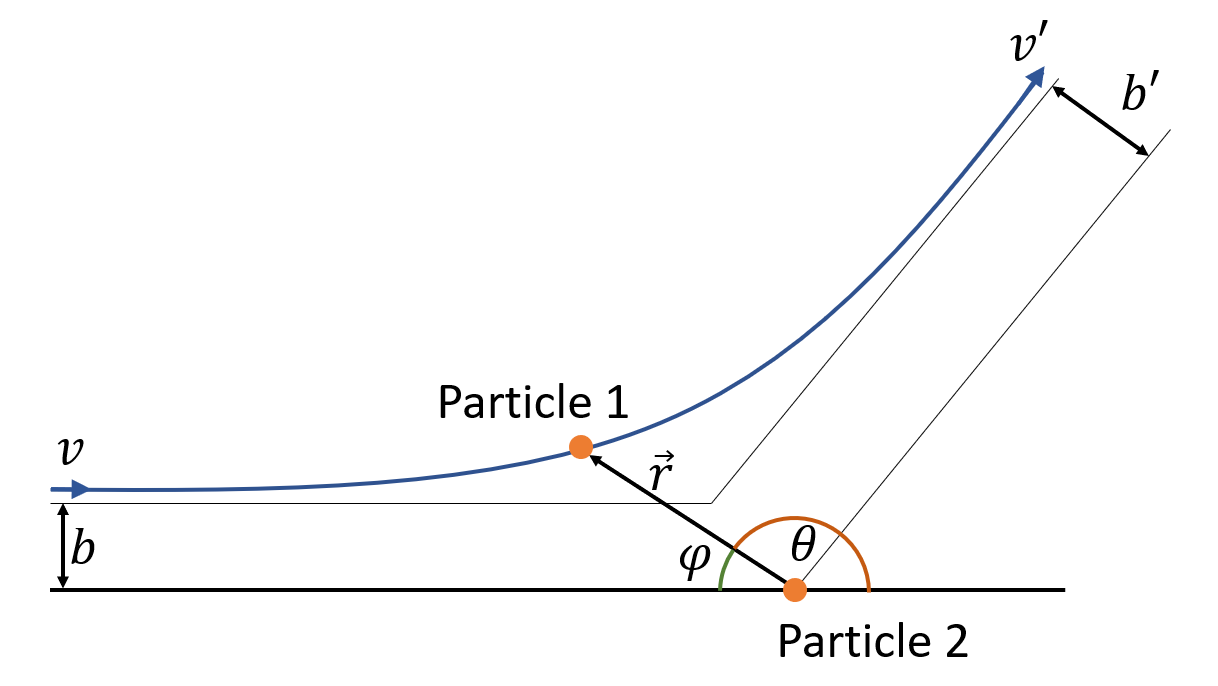
\includegraphics[width=10cm]{../../images/coulomb_scattering.png}
    \caption{Depiction of Coulomb scattering.}
    \label{fig:coulomb_scattering}
    \end{figure}

%--------------------------------------------
\subsection{Polar coordinates}
%--------------------------------------------
\begin{figure}[ht]
    \centering
    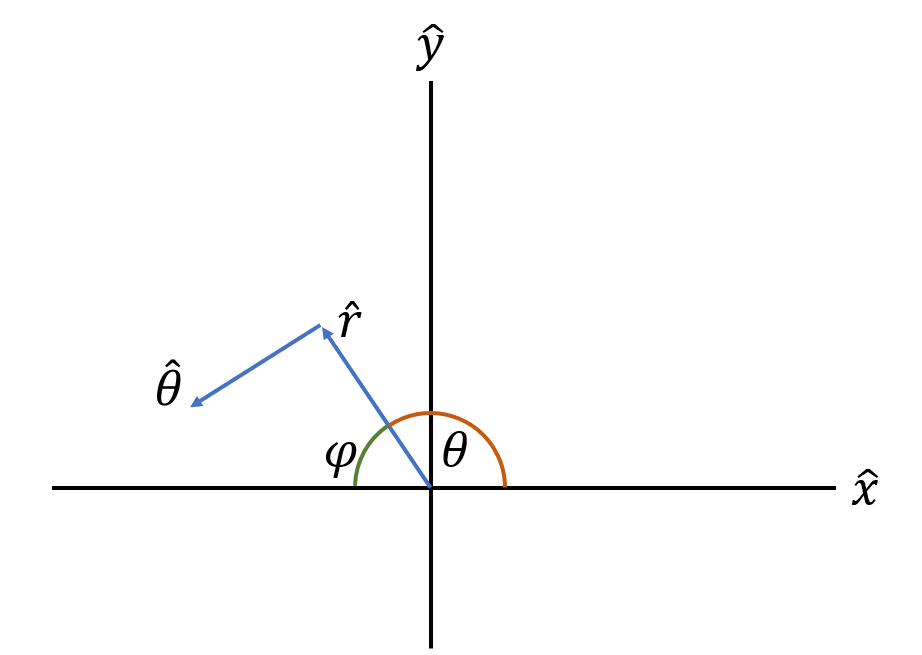
\includegraphics[width=10cm]{../../images/polar_coordinates.png}
    \caption{Polar coordinates in plane of interaction.}
    \label{fig:polar_coordinates}
    \end{figure}

We re-orient the plane of interaction (referred to above) so that it is orthogonal to the $\hat{\zvec}$ direction. Using polar coordinates, as shown in \cref{fig:polar_coordinates}, we get
\begin{equation}
    r_x = r \cos \theta = r \cos ( \pi - \varphi ) = -r \cos \varphi,
\end{equation}
\begin{equation}
    r_y = r \sin \theta = r \sin ( \pi - \varphi ) = r \sin \varphi.
\end{equation}

Also, since $\rvec = r \hat{\rvec}$, we have
\begin{align}
    \vvec = &\frac{d \rvec}{dt} = \frac{dr}{dt} \hat{\rvec} + r \frac{d\hat{\rvec}}{dt} \nonumber \\
    &= \frac{d r}{dt} \hat{\rvec} + r \frac{d\hat{\rvec}}{d\theta} \frac{d\theta}{dt} \nonumber \\
    &= \frac{dr}{dt} \hat{\rvec} + r \frac{d \theta}{dt} \hat{\bm{\theta}},
\end{align}
and
\begin{align}
    \frac{d \vvec}{dt} &= \frac{d^2r}{dt^2} \hat{\rvec} + \frac{dr}{dt} \frac{d\hat{\rvec}}{dt} + \frac{d}{dt} \left ( r \frac{d\theta}{dt} \right ) \hat{\bm{\theta}} + r \frac{d \theta}{dt} \frac{d \hat{\bm{\theta}}}{dt} \nonumber \\
    &= \frac{d^2 r}{dt^2} \hat{\rvec} + \frac{dr}{dt} \frac{d\hat{\rvec}}{d\theta} \frac{d\theta}{dt} + \frac{d}{dt} \left ( r \frac{d\theta}{dt} \right ) \hat{\bm{\theta}} + r \frac{d \theta}{dt} \frac{d \hat{\bm{\theta}}}{d\theta} \frac{d \theta}{dt} \nonumber \\
    &= \frac{d^2r}{dt^2} \hat{\rvec} + \frac{dr}{dt} \frac{d\theta}{dt} \hat{\bm{\theta}} + \frac{d}{dt} \left ( r \frac{d\theta}{dt} \right ) \hat{\bm{\theta}} - r \left ( \frac{d\theta}{dt} \right ) ^2 \hat{\rvec}.
\end{align}

%--------------------------------------------
\subsection{The force equation}
%--------------------------------------------
The radial component of \cref{eq:particle_vel} thus becomes 
\begin{equation}
    \frac{d^2 r}{dt^2} - r \left ( \frac{d\theta}{dt} \right )^2 = \frac{q_1 q_2}{4 \pi \epsilon_0 m_r} \frac{1}{r^2}.
\end{equation}
Since $\theta = \pi - \varphi$, we have
\begin{equation}
    \label{eq:particle_position_ode}
    \frac{d^2 r}{dt^2} - r \left ( \frac{d\varphi}{dt} \right )^2 = \frac{q_1 q_2}{4 \pi \epsilon_0 m_r} \frac{1}{r^2}.
\end{equation}

%--------------------------------------------
\subsection{The angular momentum equation}
%--------------------------------------------
Using polar coordinates, we obtain
\begin{equation}
    m_r \rvec \times \vvec = m_r r \hat{\rvec} \times \left ( \frac{dr}{dt} \hat{\rvec} + r \frac{d\theta}{dt} \hat{\bm{\theta}} \right ) = m_r r^2 \frac{d\theta}{dt} \hat{\zvec}
\end{equation}
Since angular momentum $m_r \rvec \times \vvec$ is conserved, we have
\begin{equation}
    \label{eq:particle_cons_angular_polar}
    m_r r^2 \frac{d\varphi}{dt} = L = constant.
\end{equation}
We note here that $L$ is positive since $d\varphi/dt$ is positive. Also, we have 
\begin{equation}
    \label{eq:particle_angular_sign}
    m_r \rvec \times \vvec = -L \hat{\zvec},
\end{equation}
that is, the angular momentum is in the negative $\hat{\zvec}$ direction.

%--------------------------------------------
\subsection{Particle trajectory}
%--------------------------------------------
The goal is to find the radial position of the particle as a function of its angular orientation. That is, we want to find $\tilde{r} = \tilde{r}(\tilde{\varphi})$ such that
\begin{equation}
    \label{eq:particle_position_angle}
    r(t) = \tilde{r}(\varphi(t)).
\end{equation}
To simplify the math, we introduce $\tilde{u} = \tilde{u}(\tilde{\varphi})$ such that $\tilde{u} = 1 / \tilde{r}$. Thus
\begin{equation}
    \frac{d \tilde{u}}{d\tilde{\varphi}} = -\frac{1}{\tilde{r}^2} \frac{d \tilde{r}}{d\tilde{\varphi}},
\end{equation}
or, after re-arranging
\begin{equation}
    \label{eq:rgrad_vs_ugrad}
    \frac{d \tilde{r}}{d\tilde{\varphi}} = -\frac{1}{\tilde{u}^2} \frac{d \tilde{u}}{d\tilde{\varphi}}.
\end{equation}

We now proceed as follows. Taking the derivative of $r$, we get
\begin{align}
    \label{eq:particle_derivation_1}
    \frac{dr}{dt} &= \left ( \frac{d \tilde{r}}{d\tilde{\varphi}} \right )_{\tilde{\varphi} = \varphi(t)} \frac{d \varphi}{dt} &&[\cref{eq:particle_position_angle}] \nonumber \\
    &= \left ( -\frac{1}{\tilde{u}^2} \frac{d\tilde{u}}{d\tilde{\varphi}} \right )_{\tilde{\varphi} = \varphi(t)} \frac{d \varphi}{dt} &&[\cref{eq:rgrad_vs_ugrad}]\nonumber \\ 
    &= \left ( -\frac{1}{\tilde{u}^2} \frac{d\tilde{u}}{d\tilde{\varphi}} \right )_{\tilde{\varphi} = \varphi(t)} \frac{L}{m_r r^2} &&[\cref{eq:particle_cons_angular_polar}] \nonumber \\
    &= \left ( -\frac{1}{\tilde{u}^2} \frac{d\tilde{u}}{d\tilde{\varphi}} \frac{L}{m_r \tilde{r}^2} \right )_{\tilde{\varphi} = \varphi(t)} &&[\cref{eq:particle_position_angle}] \nonumber \\
    &= \left ( - \frac{d\tilde{u}}{d\tilde{\varphi}} \frac{L}{m_r} \right )_{\tilde{\varphi} = \varphi(t)}
\end{align}
Taking the derivative of the above, we get
\begin{align}
    \frac{d}{dt} \frac{dr}{dt} &= \left [ \frac{d}{d\tilde{\varphi}} \left ( - \frac{d\tilde{u}}{d\tilde{\varphi}} \frac{L}{m_r} \right ) \right ]_{\tilde{\varphi} = \varphi(t)} \frac{d \varphi}{dt} \nonumber \\
    &= \left ( - \frac{d^2 \tilde{u}}{d\tilde{\varphi}^2} \frac{L}{m_r} \right )_{\tilde{\varphi} = \varphi(t)} \frac{L}{m_r r^2} && [\cref{eq:particle_cons_angular_polar}] \nonumber \\
    &= \left ( - \frac{d^2 \tilde{u}}{d\tilde{\varphi}^2} \frac{L}{m_r} \frac{L}{m_r \tilde{r}^2} \right )_{\tilde{\varphi} = \varphi(t)} && [\cref{eq:particle_position_angle}] \nonumber \\
    &= \left ( - \frac{d^2 \tilde{u}}{d\tilde{\varphi}^2} \frac{L^2 \tilde{u}^2}{m_r^2} \right )_{\tilde{\varphi} = \varphi(t)}
\end{align}
Plugging the last relation into \cref{eq:particle_position_ode} gives
\begin{equation}
    \left [ - \frac{d^2 \tilde{u}}{d\tilde{\varphi}^2} \frac{L^2 \tilde{u}^2}{m_r^2} - \frac{1}{\tilde{u}} \left ( \frac{L \tilde{u}^2}{m_r} \right )^2 \right ]_{\tilde{\varphi} = \varphi(t)} = \left ( \frac{q_1 q_2}{4 \pi \epsilon_0 m_r} \tilde{u}^2 \right )_{\tilde{\varphi} = \varphi(t)},
\end{equation}
which, upon re-arranging and dropping the $\varphi(t)$ dependance, becomes
\begin{equation}
    \frac{d^2 \tilde{u}}{d \tilde{\varphi}^2} + \tilde{u} = -\frac{q_1 q_2 m_r}{4 \pi \epsilon_0 L^2}
\end{equation}

Using \cref{eq:particle_angular_sign}, we have
\begin{align}
    \label{eq:particle_momentum_impact}
    L &= -m_r ( \rvec \times \vvec )\cdot \hat{\zvec} \nonumber \\
    &= -m_r [\sin(-\theta) r v_0 \hat{\zvec} ] \cdot \hat{\zvec} \nonumber \\
    &= m_r\sin(\theta) r v_0 \nonumber \\
    &= m_r\sin(\pi - \varphi) r v_0 \nonumber \\
    &= m_r\sin\varphi r v_0 \nonumber \\
    &= m_r b v_0.
\end{align}
Thus, we write the evolution equation for $\tilde{u}$ as
\begin{equation}
    \frac{d^2 \tilde{u}}{d \tilde{\varphi}^2} + \tilde{u} = -\frac{q_1 q_2}{4 \pi \epsilon_0 m_r b^2 v_0^2}.
\end{equation}
Introducing the notation
\begin{equation}
    b_{90} = \frac{q_1 q_2}{4 \pi \epsilon_0 m_r v_0^2},
\end{equation}
the evolution equation for $\tilde{u}$ can be simply expressed as
\begin{equation}
    \label{eq:particle_u_equation}
    \frac{d^2 \tilde{u}}{d \tilde{\varphi}^2} + \tilde{u} = -\frac{b_{90}}{b^2}.
\end{equation}

The boundary conditions for \cref{eq:particle_u_equation} are as follows
\begin{equation}
    \label{eq:particle_bc_1}
    \text{as } \varphi(t) \to 0, \quad r(t) \to \infty
\end{equation}
\begin{equation}
    \label{eq:particle_bc_2}
    \text{as } \varphi(t) \to 0, \quad \frac{dr(t)}{dt} \to -v_0
\end{equation}
Given \cref{eq:particle_position_angle}, \cref{eq:particle_bc_1} can only be satisfied if as $\tilde{\varphi} \to 0$, $\tilde{r} \to \infty$. Thus, we also have, as $\tilde{\varphi} \to 0$, $\tilde{u} \to 0$. Similarly, given \cref{eq:particle_derivation_1}, \cref{eq:particle_bc_2} can only be satisfied if as $\tilde{\varphi} \to 0$
\begin{equation}
    \frac{d\tilde{u}}{d\tilde{\varphi}} \frac{L}{m_r} \to v_0.
\end{equation}
Using \cref{eq:particle_momentum_impact} we rewrite the above as 
\begin{equation}
    \frac{d\tilde{u}}{d\tilde{\varphi}} \to \frac{1}{b}.
\end{equation}

The general solution to \cref{eq:particle_u_equation} is 
\begin{equation}
    \tilde{u} = A \cos \tilde{\varphi} + B \sin \tilde{\varphi} - \frac{b_{90}}{b^2}.
\end{equation}
Applying the boundary conditions, we get
\begin{equation}
    \tilde{u} = \frac{b_{90}}{b^2} \cos \tilde{\varphi} + \frac{1}{b} \sin \tilde{\varphi} - \frac{b_{90}}{b^2},
\end{equation}
which we finally re-write as
\begin{equation}
    \frac{1}{\tilde{r}} = \frac{1}{b} \sin \tilde{\varphi} + \frac{b_{90}}{b^2} \left ( \cos \tilde{\varphi} - 1 \right ).
\end{equation}


